\documentclass{article}
\usepackage{afterpage}
\usepackage{amsmath}
\usepackage{amssymb}
\usepackage[page,toc,titletoc,title]{appendix}
\usepackage{array}
\usepackage{authblk}
\usepackage{bbold}
\usepackage[backend=biber,style=alphabetic,sorting=ynt]{biblatex}
\usepackage{booktabs}
\usepackage[font=footnotesize]{caption}
\usepackage{capt-of}
\usepackage{float}
\usepackage{hyperref}
\hypersetup{
    colorlinks=true,
    linkcolor=blue,
    filecolor=magenta,      
    urlcolor=violet,
    citecolor=violet,
    pdftitle={Simulations of qubit communication in prepare-and-measure and Bell scenarios},
    pdfpagemode=FullScreen,
}
\usepackage{graphicx}
\graphicspath{ {./images/} }
\usepackage{lscape}
\usepackage{longtable}
\usepackage{msc}
\usepackage{minted}
\usepackage{multirow}
\usepackage[skip=7pt plus1pt, indent=20pt]{parskip}
\usepackage{pdflscape}
\usepackage{physics}
\usepackage{subcaption}
\usepackage{svg}
\usepackage{tikz}
\usetikzlibrary{quantikz}
\usepackage{xcolor}
\usepackage{xurl}
\addbibresource{bibliography.bib}

\begin{document}

\begin{titlepage}
   \begin{center}
       \vspace*{1cm}

       \Large
       \textbf{Simulations of qubit communication in prepare-and-measure and Bell scenarios}

       \vspace{0.8cm}

       \normalsize
       \textbf{I\~{n}aki Ortiz de Landaluce S\'aiz\\Aido Cort\'es Alcar\'az\\}
       \vspace{0.5cm}
       \footnotesize{Supervised by Gael Sent\'is Herrera (Universitat Aut\`onoma de Barcelona)}
       \vfill
            
       \footnotesize{A project submitted for the Postgraduate Degree in Quantum Engineering}
            
       
\includegraphics[width=0.8\textwidth]{images/upc.png}
            
       \date{\today}
            
   \end{center}
\end{titlepage}
\newpage
\renewcommand{\abstractname}{Abstract}
\begin{abstract}
In the early years of the current century, a breakthrough was made in Quantum Information Theory by David Bacon and Ben Toner, who developed a quantum communication protocol showing that any prediction based on projective measurements (PVMs) on a qubit could be simulated by communicating only two classical bits. This result has been very recently extended by Martin Renner, Armin Tavakoli and Marco Tulio Quintino to positive operator-valued measures (POVMs) without any loss of generalisation, keeping the classical cost of a qubit transmission still as two bits. In this project we have simulated such extended protocol classically and compared its outcomes against a quantum simulator and a noisy intermediate-scale quantum computer, to show how two bits of communication are enough to reproduce all quantum correlations associated to arbitrary POVMs applied to any prepare-and-measure scenario, and also to any entangled two-qubit pair state. With this investigation we give rise to explore and understand computationally some fundamental limits of quantum over classical advantages.
\end{abstract}
\newpage
\tableofcontents

\newpage
\section{Introduction}
\subsection{Objective}
Quantum information theory provides a framework to quantify the power of quantum theory compared to Shannon's classical communication theory \cite{shannon}. Over the last decades, the field has flourished compelled to set realistic boundaries to the promises of quantum advantages in fields like quantum communication and computing. An important feature of quantum theory lies in the statistical correlations produced by local measurements of a quantum system. The simplest example of quantum correlations are the ones produced by projective measurements on a maximally-entangled state of two qubits, also known as a Bell pair state. Such correlations are the basic resource of bipartite quantum information theory, where various equivalences are known: one shared Bell pair plus two bits of classical information can be used to teleport one  qubit and, conversely, one shared Bell pair state plus a single qubit can be used to send two bits of classical information via superdense coding. Exploring the fundamental limits of quantum over classical advantages in these scenarios is crucial, and it will be the primary objective of this work.
\par
In the early years of the current century, Ben Toner and David Bacon developed a protocol which proves that any prediction based on projective measurements on an entangled Bell pair state could be simulated by communicating only two classical bits \cite{toner2003}. Very recently, Martin Renner, Armin Tavakoli and Marco Tulio Quintino, have extended such result to a most generalised set of measurements, the positive operator-valued measures \cite{renner2022}.
Following up such generalization, we will show via computer-based experiments that a qubit transmission can be simulated classically with a total cost of two bits for any general measurement, either in a prepare-and-measure or an entanglement scenario. This will prove experimentally that the protocols described in \cite{renner2022} can be reproduced computationally using classical computers, and that the probability distributions obtained can be compared against the ones resulting from performing generalized measurements with existing quantum simulators and noisy intermediate-scale quantum computers.
\par
Before starting to describe the different computational experiments we have carried out to achieve such goal, it is worth spending next sections to introduce some preliminary concepts and notations that have been used extensively throughout this work, specifically the definition of positive operator-valued measures, the set-up of both the prepare-and-measure and Bell scenarios and the particular details of the classical simulation protocols applied to such scenarios.
\par
\subsection{Positive operator-valued measures}\label{section:povms}
Even when most of the introductory textbooks on quantum mechanics describe the measurement postulates using projective measurements only, there exists a more general and less restrictive set of measurements called Positive Operator-Valued Measures or POVMs, see \cite{nielsen2000}\cite{peres1995}. The underlying formalism behind POVMs is uniquely well adapted for some applications where the main focus is on describing the probabilities of the different measurement outcomes rather than on the post-measurement state of the system. This is of particular interest in quantum communication and quantum information, where a more comprehensive formalism for the description of the measurements is needed, and highlights how important are the results from \cite{renner2022}, where all the results are extended to POVMs without any loss of generalisation regarding the the classical simulation cost of the protocol. For reference, we define explicitely a POVM as a set $\mathbb{P}=\{B_{k}\}$ of $k=1,...,N$ positive semidefinite operators acting on a Hilbert space $\mathcal{H}$ of dimension $d_{Q}$, which satisfies the closure property $\sum_{k=1}^{N} B_{k} = \mathbb{1}$. The operator $B_{k}$ is called a POVM element, and it is associated to the outcome $k$ of the POVM. In this work we will use extensively the property which states that every qubit POVM can be written as a coarse graining of rank-1 projectors \cite{barrett2002}, such that we will restrict our POVM calculations to the case of rank-1 projectors.

\subsection{Prepare-and-measure scenario}\label{section:pm}
As for many other communication protocols we have two well-known characters playing different roles in the quantum prepare-and-measure set-up: Alice and Bob. The prepare-and-measure scenario starts with Alice preparing a random quantum state and sending it to Bob. In a general set-up, i.e. not restricted to single qubit communication, the state prepared by Alice is a state of dimension $d_Q$ described by a positive semidefinite density matrix $\rho \in \mathcal{L}( \mathbb{C}_{d_Q}), \rho \ge 0$ with unit trace $tr(\rho)=1$. Once the state is prepared and communicated by Alice, Bob then receives it and performs a random quantum measurement on it, obtaining an outcome $k$. In the case of general POVM measurements $\mathbb P=\{B_{k}\}$ as described in Section \ref{section:povms}, the probability of outcome $k$ when performing the measurement on the state $\rho$ is given by Born's rule,

\begin{equation}\label{eq:prob_quantum}
p_Q(k|\rho,\{B_{k}\}) = tr(\rho B_{k})
\end{equation}

In the context of this work, we are interested in the classical counterpart of the quantum prepare-and-measure scenario, where the probability distributions predicted by the quantum theory (\ref{eq:prob_quantum}) are reproduced classically. All these classical counterparts of existing quantum protocols, see examples in \cite{cerf2000}, \cite{toner2003} and \cite{renner2022}, require a shared randomness $\lambda$ among Alice and Bob subject to some probability function $\pi(\lambda)$ to correlate their classical communication strategies. As it is not possible to reproduce these correlations without communication, a classical message $c$ which encodes classically the quantum state $\rho$ taking its value from a $d_C$-valued alphabet $\{1,...,d_C\}$ is also required. Alice's actions are therefore described by the conditional probability $p_A(c|\rho,\lambda)$, whereas Bob's actions are similarly described by the conditional probability $p_B(k|\{B_{k}\},c,\lambda)$. If we consider both probabilities, the correlations from the classical counterpart become

\begin{equation}\label{eq:prob_classic}
p_C(k|\rho,\{B_{k}\}) = \int_{\lambda} d\lambda\ \pi(\lambda) \sum_{c=1}^{d_C} p_A(c|\rho, \lambda)\ p_B(k|\{B_{k}\}, c, \lambda)
\end{equation}

Given Equations (\ref{eq:prob_quantum}) and (\ref{eq:prob_classic}), the classical simulation would be considered successful when, for every random state and POVM, the classical probability distribution reproduces the quantum predictions, i.e.

\begin{equation}\label{eq:prob_classic_quantum}
\forall \rho, \{B_{k}\}:\quad p_C(k|\rho,\{B_{k}\}) = p_Q(k|\rho,\{B_{k}\})
\end{equation}

\subsection{Bell scenario}
In a Bell scenario, there is a bipartite quantum system of two entangled and separated qudits, one with Alice and another one with Bob. 
Alice chooses a random local measurement $A_x$ among two possible observables $\{A_0, A_1\}$, and produces an output $a_x$ according to the distribution of her measurement elements. Following the same procedure, Bob chooses his own random local measurement $B_y$, among two possible observables $\{B_0, B_1\}$, and produces an outcome $b_y$. Even if both outcomes appear random, their joint probabilities $p_{A_x,B_y}(a_x, b_y)$ are correlated. We refer to these correlations as Bell correlations. 

Similarly to the prepare-and-measure case described in Section \ref{section:pm}, it is not possible to reproduce the correlations using a classical protocol with shared random variables without allowing classical communication among Alice and Bob once they have selected their measurements, see \cite{bell1964}. The main question here is to determine how much classical communication is needed to reproduce the probability distributions.

As \cite{renner2022} shows, it is straight-forward to adapt the prepare-and-measure classical scenario to any entangled qudit-qubit state. Here Alice chooses a random local POVM on a $d_Q$-dimensional quantum system, and produces an output according to the marginal distribution of her POVM elements. Based on her output, she computes Bob's entangled qubit post-measurement state, which is sent to Bob using the prepare-and-measure scenario. Given that Bob's post-measurement qubit state is communicated by Alice using the existing prepare-and-measure classical protocol, the classical cost of the qubit transmission will be exactly the same: two bits. 

In addition, we can restrict our quantum system to a bipartite state of two qubits and local and projection valued measures. The maximally entangled states in such scenario are the well-known Bell states $\ket{\Phi_{ij}}$, as follows
\begin{equation}\label{eq:bell_states}
\begin{split}
\ket{\Phi^{+}} \vcentcolon= \frac{1}{\sqrt{2}}(\ket{00} + \ket{11})\\
\ket{\Phi^{-}} \vcentcolon= \frac{1}{\sqrt{2}}(\ket{00} - \ket{11})\\
\ket{\Psi^{+}} \vcentcolon= \frac{1}{\sqrt{2}}(\ket{01} + \ket{10})\\
\ket{\Psi^{-}} \vcentcolon= \frac{1}{\sqrt{2}}(\ket{01} - \ket{10})
\end{split}
\end{equation}
Each local projective measurements has two eigenvalues, either $\ket{a_{x}}$ or $\ket{b_{y}}$, with outcomes $a_{x}, b_{y}=\pm1$ respectively. In this scenario, the joint probabilities can be defined as
\begin{equation}\label{eq:prob_quantum_bell}
\begin{split}
p_{A_x,B_y}(a_x, b_y) = tr[\ket{a_{x}}\bra{a_{x}} \otimes \ket{b_{y}}\bra{b_{y}} \ket{\Phi_{ij}} \bra{\Phi_{ij}}]\\
\end{split}
\end{equation}

The expected values for a given set of observables $(A_{x}, B_{y})$ can be defined from the joint probabilities as follows
\begin{equation}\label{eq:bell_expected_values}
\begin{split}
\mathbb{E}[A_{x}, B_{y}] \vcentcolon= p_{A_x,B_y}(+1, +1)\,- p_{A_x,B_y}(+1, -1)\\-p_{A_x,B_y}(-1, +1)\,+ p_{A_x,B_y}(-1, -1)
\end{split}
\end{equation}
which also leads to the famous Clauser-Horne-Shimony-Holt expression
\begin{equation}\label{eq:bell_inequality}
CHSH \vcentcolon= \mathbb{E}[A_{0},B_{0}]\,+\mathbb{E}[A_{1},B_{0}]\,+\mathbb{E}[A_{0},B_{1}]\,-\mathbb{E}[A_{1},B_{1}]
\end{equation}

The classical protocol described in [RTQ22] using a Bell singlet state $\ket{\Psi^{-}}$, proves that a classical communication of one single bit is enough to reproduce the joint probabilities when Alice performs projective measurements an Bob can either perform projective or positive operator-valued measurements. Similarly as in the prepare and measure scenario, the classical probability distribution can be defined as
\begin{equation}\label{eq:prob_classic_bell}
p_C(a_{x}, b_{y}|A_{x},B_{y}) = \int_{\lambda} d\lambda\ \pi(\lambda) p_A(c|A_{x}, \lambda)\ p_B(b_{y}|B_{y}, c, \lambda)
\end{equation}

Given Equations (\ref{eq:prob_quantum_bell}) and (\ref{eq:prob_classic_bell}), the classical simulation would be considered successful when, given a bipartite singlet state $\ket{\Psi^{-}}$, for every set of observables $\{A_{x}, B_{y}\}$, the classical probability distribution reproduces the quantum predictions, i.e.

\begin{equation}\label{eq:prob_classic_quantum_bell}
\forall A_{x}, B_{y}:\quad p_C(a_{x}, b_{y}|A_{x},B_{y}) = p_{A_x,B_y}(a_x, b_y)
\end{equation}

\subsection{Classical simulation protocols}\label{section:protocols}
\subsubsection{Prepare-and-measure with one qubit}\label{section:protocol_pm}
The classical prepare-and-measure protocol proposed by Renner, Tavakoli and Quintino \cite{renner2022} is restricted to qubits ($d_Q=2$), and makes an extensive use of the geometrical properties of a qubit state in the Bloch sphere. Since mixed qubit states are convex combinations of pure states, the protocol is also restricted to the usage of pure states only. Toner and Bacon proved that making a further restriction to projective measurements, i.e. $B_{k}^{2} = B_{k}$, the classical simulation cost was upper bounded by two classical bits ($d_C=2$) \cite{toner2003}, but \cite{renner2022} generalizes the results to positive operator-valued measures with a minimal and therefore necessary classical cost of two qubits. Finally, the protocol is also restricted without any loss of generality to POVMs proportional to rank-1 projectors, following results in \cite{barrett2002}.

In Bloch notation, qubit states $\rho$ are represented by three-dimensional real normalized vectors $\vec{x} \in \mathbb{R}^{3}$, and rank-1 POVM projectors as 
\begin{equation}\label{eq:rank1_povm}
B_{k} = 2p_{k}\ket{\vec{y}_{k}}\bra{\vec{y}_{k}}
\end{equation}
where $p_{k}\ge0,\ \sum_{k=1}^{N}p_{k}=1$ and $\ket{\vec{y}_{k}}\bra{\vec{y}_{k}} = (\mathbb{1} + \vec{y}_{k} \cdot \vec{\sigma})/2$ for some normalized vector $\vec{y}_{k} \in \mathbb{R}^{3}$, such that

\begin{equation}
tr(\rho B_{k}) = p_{k}(1 + \vec{x} \cdot \vec{y}_{k}) 
\end{equation}

Two additional functions need to be defined prior to make the classical protocol steps explicit, these are the Heaviside function
\begin{equation}
H(z) =
    \begin{cases}
      1 & \text{when $z \ge 0$}\\
      0 & \text{when $z<0$}
    \end{cases} 
\end{equation}
and $\Theta(z) := z \cdot H(z)$. Under all these considerations, the protocol, as defined in \cite{renner2022} and sketched in Figure \ref{fig:msc_pm}, is literally as follows:
\begin{enumerate}
 \item Alice and Bob share two normalized vectors $\vec{\lambda}_1, \vec{\lambda}_2 \in \mathbb{R}^{3}$, which are uniformly and independently distributed on the unit radius sphere $S_2$.
 \item Instead of sending a pure qubit $\rho = (\mathbb{1} + \vec{x} \cdot \vec{\sigma})/2$, Alice prepares two bits via the formula $c_1= H(\vec{x} \cdot \vec{\lambda}_1)$ and $c_2= H(\vec{x} \cdot \vec{\lambda}_2)$ and sends them to Bob.
 \item Bob flips each vector $\vec{\lambda}_i$ when the corresponding bit $c_i$ is zero. This is equivalent to set $\vec{\lambda}^{\prime}_{i} := (-1)^{1 + c_i} \vec{\lambda}_{i}$.
 \item Instead of performing a POVM with elements $B_{k} = 2p_{k}\ket{\vec{y}_{k}}\bra{\vec{y}_{k}}$, Bob picks one vector $\vec{y}_{k}$ from the set $\{\vec{y}_{k}\}$ according to the probabilities $\{p_{k}\}$. Then he sets $\vec{\lambda} := \vec{\lambda}^{\prime}_1$ if $\lvert \vec{\lambda}^{\prime}_1 \cdot \vec{y}_{k} \rvert \ge \lvert \vec{\lambda}^{\prime}_2 \cdot \vec{y}_{k} \rvert$ and $\vec{\lambda} := \vec{\lambda}^{\prime}_2$ otherwise. Finally, Bob outputs $k$ with probability
\end{enumerate}

\begin{equation}\label{eq:prob_classic_bob}
p_B(k|\{B_{k}\},\vec{\lambda}) = \frac{p_{k}\ \Theta(\vec{y}_{k} \cdot \vec{\lambda})}{\sum_{j}^{N}p_j\ \Theta(\vec{y}_j \cdot \vec{\lambda})}
\end{equation}

\begin{figure}[tb]
\begin{center}
\begin{msc}[msc keyword=, instance width=3.6cm]{Prepare-and-measure classical protocol}
\declinst{alice}{}{Alice}
\declinst{bob}{}{Bob}
\condition*{shared randomness $\vec{\lambda}_1, \vec{\lambda}_2$}{alice,bob}
\nextlevel[3]
\action*{$c_i = H(\vec{x} \cdot \vec{\lambda_i})$}{alice}
\nextlevel[3]
\mess{$c_1, c_2 \in \{0,1\}$}{alice}{bob}
\nextlevel[1]
\action*{$\vec{\lambda}^{\prime}_i = (-1)^{1 + c_i} \vec{\lambda_i}$}{bob}
\nextlevel[3]
\action*{$p_B(k|\{B_{k}\},\vec{\lambda})$}{bob}
\nextlevel[2]
\end{msc}
\end{center}
\caption{Classical prepare-and-measure protocol sequence: Alice sends two bits $c_1, c_2$ resulting from projecting the qubit state's Bloch vector $\vec{x}$ with respect to the shared random vectors $\vec{\lambda}_1, \vec{\lambda}_2$ through a classical channel, Bob flips the shared random vectors when necessary, and finally computes classical probability outcomes according to Equation (\ref{eq:prob_classic_bob}).}
\label{fig:msc_pm}
\end{figure}

%https://tex.stackexchange.com/questions/368604/how-to-draw-a-half-and-half-colored-circle
%\pgfmathsetmacro{\radius}{2}
%\begin{tikzpicture}
%    %\fill[gray!50,opacity=0.7] (0,0) circle (\radius); 
%    %\fill[gray!10, opacity=1] (0,0) -- (135:\radius) arc (135:315:\radius) -- cycle; 
%    \draw[] circle(\radius);
%    \draw[thick,->] (0,0,0) -- (\radius,0,0) node[anchor=north west]{$\vec{\lambda}_1$};
%    \draw[thick,->] (0,0,0) -- (-0.3473, 1.9696,0) node[anchor=south east]{$\vec{\lambda}_2$};
%    \draw[thick,->] (0,0,0) -- (1.4142, 1.4142,0) node[anchor=south]{$\vec{x}$};
%    \draw[dashed] (-1.414,1.414,0) -- (1.414,-1.414,0) node[anchor=south]{};    
%\end{tikzpicture}

%\tdplotsetmaincoords{40}{0}
%\tdplotsetrotatedcoords{150}{50}{20}
%\begin{tikzpicture}[scale=2,line join=bevel,tdplot_rotated_coords,fill %opacity=1,declare function={ colorFunc(\t)=ifthenelse(\t>0,60,300);}]
%\pgfsetlinewidth{.0pt}
%    \tdplotsphericalsurfaceplot[parametricfill]{72}{36}{2}%{transparent!0}{colorFunc(180*floor(\tdplotphi/180))
%    }{}{}{}
%\end{tikzpicture}

\subsubsection{Bell with singlet state}\label{section:protocol_bell}
Toner a Bacon showed in \cite{toner2003} that only a single bit was required to classically simulate local projective measurements on a qubit pair in a singlet state $\ket{\psi^{-}}=\frac{1}{\sqrt{2}}(\ket{01} - \ket{10})$. Renner, Tavakoli and Quintino again extended such result being Alice restricted to local projective measurements with outcomes $a=\pm 1$, and Bob allowed to perform any arbitrary POVM measure \cite{renner2022}. The steps for this protocol, sketched in Figure \ref{fig:msc_bell}, are the following:
\begin{enumerate}
 \item Alice and Bob share two normalized vectors $\vec{\lambda}_1^{\prime}, \vec{\lambda}_2 \in \mathbb{R}^{3}$, which are uniformly and independently distributed on the unit radius sphere $S_2$.
 \item Instead of performing a measurement with projectors $\ket{\pm\vec{x}}\bra{\pm\vec{x}} = (\mathbb{1} + \vec{x} \cdot \vec{\sigma})/2$, Alice outputs $a = -sgn(\vec{x} \cdot \vec{\lambda}^{\prime}_1)$ and sends the bit $c = sgn(\vec{x} \cdot \vec{\lambda}^{\prime}_1) \cdot sgn(\vec{x} \cdot \vec{\lambda}_2)$ to Bob, where 
 \begin{equation}
sgn(z) =
    \begin{cases}
      1 & \text{when $z \ge 0$}\\
      -1 & \text{when $z<0$}
    \end{cases} 
\end{equation}
 \item Bob flips the vector $\vec{\lambda}_2$ if and only if $c=-1$, i.e. he sets $\vec{\lambda}^{\prime}_{2} := c \vec{\lambda}_{2}$.
 \item Same as step 4 in the previous prepare-and-measure protocol.
\end{enumerate}

\begin{figure}[tb]
\begin{center}
\begin{msc}[msc keyword=, instance width=3.6cm]{Bell with singlet state classical protocol}
\declinst{alice}{}{Alice}
\declinst{bob}{}{Bob}
\condition*{shared randomness $\vec{\lambda}_1^{\prime}, \vec{\lambda}_2$}{alice,bob}
\nextlevel[3]
\action*{$c = sgn(\vec{x} \cdot \vec{\lambda}^{\prime}_1) \cdot sgn(\vec{x} \cdot \vec{\lambda}_2)$}{alice}
\nextlevel[3]
\mess{$c \in \{-1,1\}$}{alice}{bob}
\nextlevel[1]
\action*{$\vec{\lambda}^{\prime}_2 = c \vec{\lambda_2}$}{bob}
\nextlevel[3]
\action*{$p_B(k|\{B_{k}\},\vec{\lambda})$}{bob}
\nextlevel[2]
\end{msc}
\end{center}
\caption{Classical Bell with singlet state protocol sequence: Alice sends one bit $c$ resulting from projecting the associated projective measurement's Bloch vector $\vec{x}$ with respect to the shared random vectors $\vec{\lambda}_1, \vec{\lambda}_2$ through a classical channel, Bob flips the shared random vectors when necessary, and finally computes classical probability outcomes according to the response function from the prepare-and measure protocol, see Equation (\ref{eq:prob_classic_bob}).}
\label{fig:msc_bell}
\end{figure}

It can be proved that when Alice outputs $a=+1$, $\vec{\lambda}^{\prime}_1$ and $\vec{\lambda}^{\prime}_2$ are distributed on $S_2$ according to $\rho(\vec{\lambda}^{\prime}_i) = H(-\vec{x} \cdot \vec{\lambda}^{\prime}_i)/(2\pi)$, which corresponds to a classical description of Bob's post-measurement state $-\vec{x}$ and, conversely, when Alice outputs $a=-1$, the random vectors are distributed according to a distribution corresponding to Bob's post-measurement state $\vec{x}$, and therefore Bob can apply the same response function as in the prepare-and-measure protocol described in \ref{section:protocol_pm}. 
\newpage
\section{Methodology\label{section:methodology}}
In this section we will discuss the different methods required to effectively run classical computational simulations of the protocols described in Section \ref{section:protocols} such that, for any choice of qubit pure states and rank-1 POVMs, the quantum predictions in Eq. (\ref{eq:prob_quantum}) are reproduced classically following Eq. (\ref{eq:prob_classic}), i.e.
\begin{equation}
\forall \rho, \{B_{k}\}:\quad tr(\rho B_{k}) = \int_{\lambda} d\lambda\ \pi(\lambda) \sum_{c=1}^{d_C} p_A(c|\rho, \lambda)\ p_B(k|\{B_{k}\}, c, \lambda)    
\end{equation}
and for a Bell singlet state $\ket{\Psi^{-}}$ and any choice of PVMs, the quantum predictions in Eq. (\ref{eq:prob_quantum_bell}) are reproduced classically following Eq. (\ref{eq:prob_classic_bell}), i.e.
\begin{equation}
\forall A_{x}, B_{y}: |\bra{\Psi_{ij}}\ket{a_{x}} \otimes \ket{b_{y}}|^{2} = \int_{\lambda} d\lambda\ \pi(\lambda) p_A(c|A_{x}, \lambda)\ p_B(b_{y}|B_{y}, c, \lambda)
\end{equation}


The main goal is to carry out these simulations using standard classical computations, but some particular results will be confronted with the outcomes from quantum circuit simulators and quantum computers, therefore there will be specific subsections devoted to the implementation of generalized measurements in a quantum circuit model. 
\subsection{State preparation}
In the classical simulations, the state preparation would require to produce a random qubit pure state first, and then to compute the corresponding Bloch vector to be used later by Alice. 

In the prepare-and-measure scenario, Alice uses the Bloch vector representation of the qubit's pure state, and Bob's POVMs,  proportional to rank-1 projectors, are expressed as the outer product of the associated Bloch vectors. In the Bell scenario, Alice also uses the Bloch vector corresponding to the local projective measurement projectors. In addition, in all these protocols, Alice and Bob share two random normalized vectors $\vec{\lambda}_1, \vec{\lambda}_2 \in \mathbb{R}^{3}$, which must be uniformly and independently distributed on the unit sphere $S_2$, which is analogous to generate random Bloch vectors in the Bloch sphere. Given the fact that the classical probabilities obtained with the different protocols must be equivalent to the quantum probabilities for any state and POVM measure, and that generating a true shared randomness is a fundamental element of the classical protocols, it is of key importance to be able prepare random normalized vectors uniformly distributed along the unit radius sphere $S_2$. Hence, the randomized qubit state preparation in the form of Bloch vectors is not only the building block for the state preparation itself, but plays also a critical role in the measurement construction and the shared randomness creation.

To produce a random qubit pure state we should obtain a random unitary matrix and then apply the unitary transformation to the zero qubit state, resembling the time evolution of a qubit from a zero initial state. The random unitary matrix can be generated by just building a matrix of normally distributed complex numbers, and then apply the Gram-Schmidt QR decomposition to orthogonalize the matrix, see \cite{ozols2009}, \cite{zyczkowski1994}. 

The resulting random qubit state distribution can be validated using the corresponding Bloch vector distribution along the unit radius sphere. A tessellation scheme called HEALPix \cite{healpix}, which produces a hierarchical and equal-area iso-latitude pixelation of a sphere, could be used to show that the random Bloch vectors are uniformly and independently distributed in the Bloch sphere. Given that each pixel in HEALPix covers the same surface area as every other pixel (see Figure \ref{fig:healpix_sphere}), we can group the Bloch vector distribution along the different pixel indices (see Figure \ref{fig:healpix_numbering}), and check whether the resulting distribution is uniform as expected.

\begin{figure}[!ht]
\begin{center}
\centerline{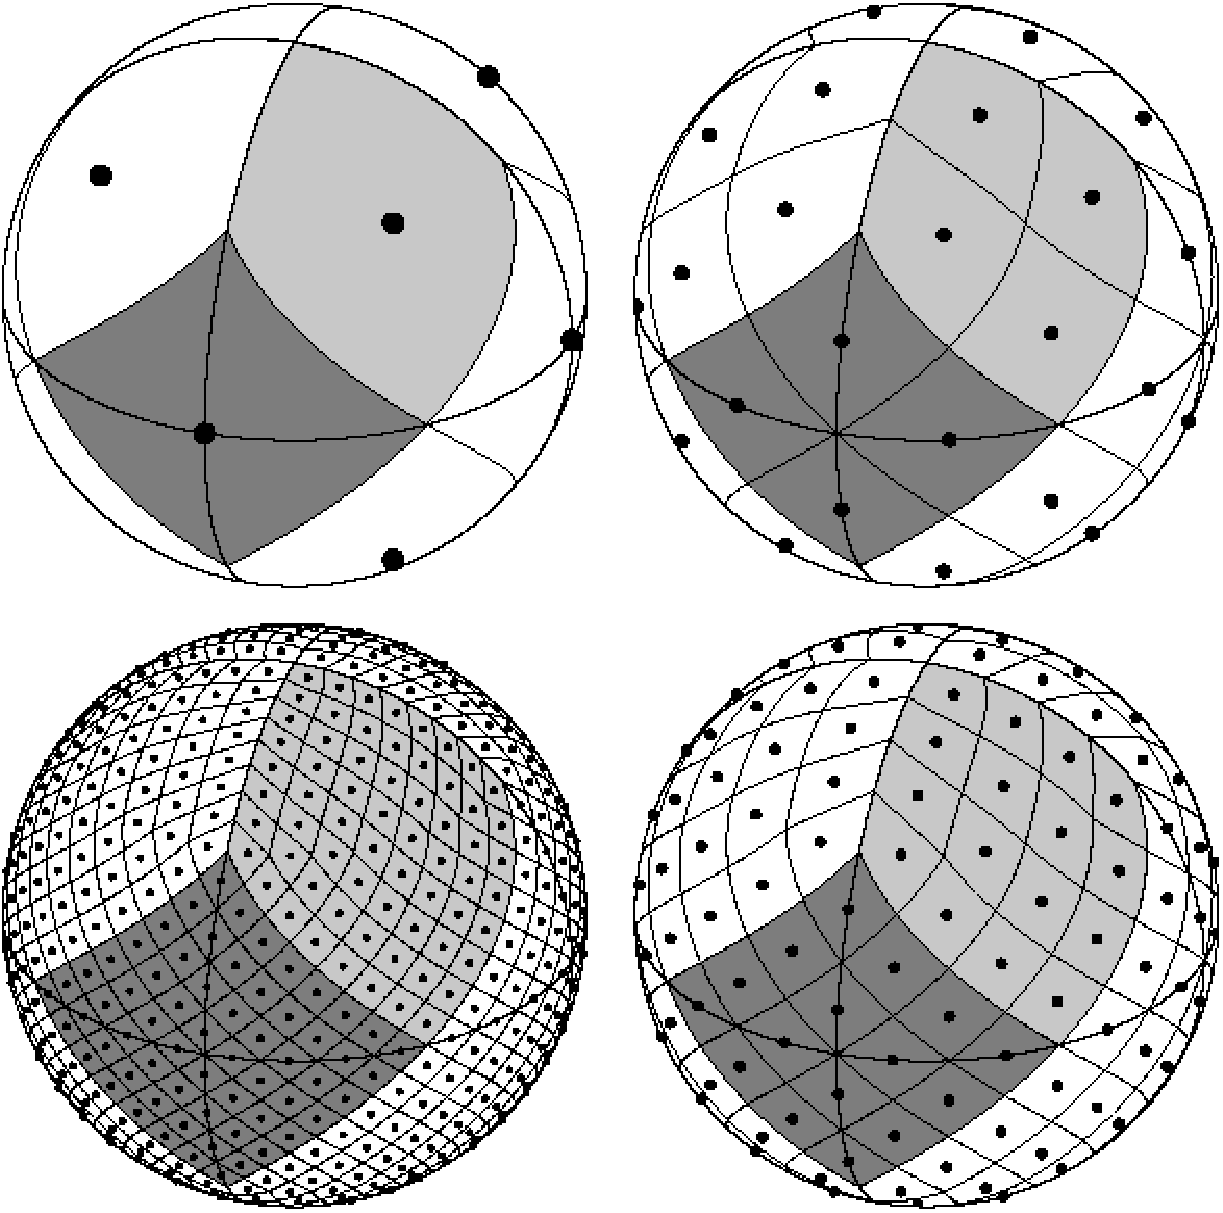
\includegraphics[height=5.5cm]{images/healpix4.pdf}}
\caption[Orthographic view of Healpix partition of the sphere]%
{\label{fig:healpix_sphere}%
Orthographic view of HEALPix partition of the sphere.}
\end{center}
\end{figure}

\begin{figure} [!ht]
\begin{center}
\centerline{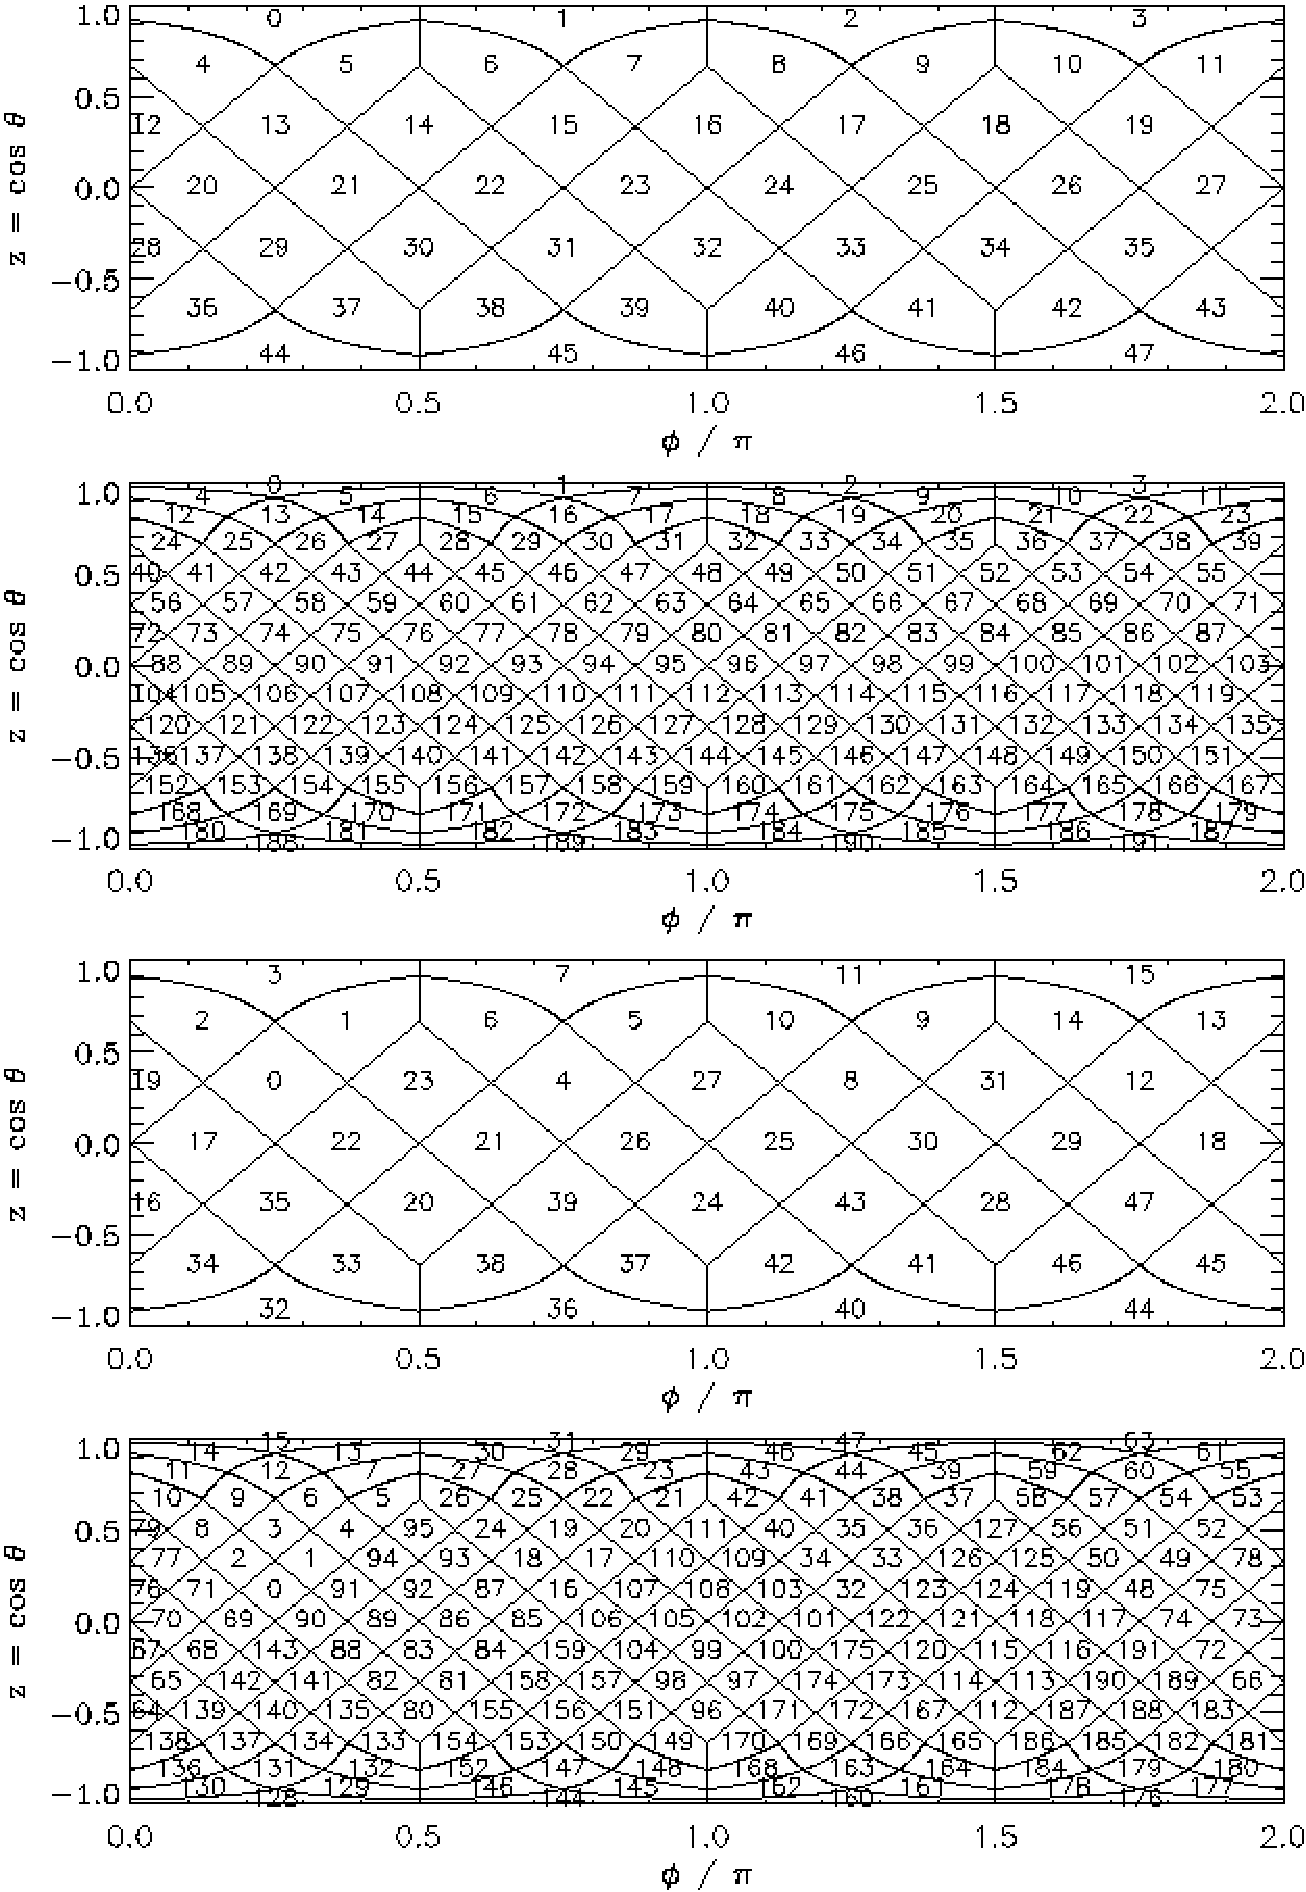
\includegraphics[height=10.5cm]{images/healpix2d.pdf}}
\caption[Cylindrical projection]%
{\label{fig:healpix_numbering}%
Cylindrical projection of the HEALPix division of a
sphere and two natural pixel numbering schemes (RING and NESTED). 
Both numbering schemes map the two dimensional 
distribution
of discrete area elements on a sphere into the one dimensional, 
integer pixel number array.
}
\end{center}
\end{figure}
\subsection{Rank-1 POVMs implementation}
We have already discussed how every qubit POVM can be written as a coarse graining of rank-1 projectors \cite{barrett2002}, such that the protocol implementation can restrict without any loss in generality to POVMs proportional to rank-1 projectors. 

Even if the final goal is to build POVMs to test how the classical protocol converges with the quantum theory for any random state and measurement, we will also discuss some general rank-1 POVMs with interesting properties, for example, 
\begin{enumerate}
    \item The measure needed in the eavesdropping  of the BB84 protocol \cite{nielsen2000}
\begin{equation}\label{eq:cross-povm}
    \mathbb{P}_4 = \{\frac{1}{2}\ket{0}\bra{0}, \frac{1}{2}\ket{1}\bra{1}, \frac{1}{2}\ket{+}\bra{+}, \frac{1}{2}\ket{-}\bra{-} \}
\end{equation}
    \item The Trine-POVM, consisting of POVM elements uniformly distributed on an equatorial plane of the Bloch sphere, with $\mathbb{P}_3=\{E_1, E_2, E_3\}$ and $E_k=\frac{2}{3}\ket{\Psi_{k}}\bra{\Psi_{k}}$, where
\begin{equation}\label{eq:trine-povm}
\begin{split}
\ket{\Psi_1}&=\ket{0}\\
\ket{\Psi_2}&=\frac{1}{2}\ket{0} + \frac{\sqrt{3}}{2} \ket{1}\\ 
\ket{\Psi_3}&=\frac{1}{2}\ket{0} - \frac{\sqrt{3}}{2} \ket{1}
\end{split}
\end{equation}
    \item The SIC-POVMs, a well-known family of symmetric informationally complete positive operator-valued measures, which are proven to be very relevant in quantum state tomography and quantum cryptography fields among others \cite{renes2004}. The simplest SIC-POVM is the one with states the vertices of a regular tetrahedron in the Bloch sphere, see Figure \ref{fig:sic_povm}, with $\mathbb{P}_4=\{E_1, E_2, E_3, E_4\}$ and $E_k=\frac{1}{2}\ket{\Psi_{k}}\bra{\Psi_{k}}$, where
\begin{equation}\label{eq:sic-povm}
\begin{split}
\ket{\Psi_1}&=\ket{0}\\ 
\ket{\Psi_2}&=\frac{1}{\sqrt{3}}\ket{0} + \sqrt{\frac{2}{3}} \ket{1}\\
\ket{\Psi_3}&=\frac{1}{\sqrt{3}}\ket{0} + \sqrt{\frac{2}{3}} \ e^{i\frac{2\pi}{3}} \ket{1}\\ 
\ket{\Psi_4}&=\frac{1}{\sqrt{3}}\ket{0} + \sqrt{\frac{2}{3}}\ e^{i\frac{4\pi}{3}} \ket{1}
\end{split}
\end{equation}
\end{enumerate}

The strategies to build the rank-1 POVMs and perform the measurement are different in the classical simulation protocol and in the quantum circuit model, as we will see later, so next sections will describe the methodologies applied for each case.

\begin{figure}[!ht]
\begin{center}
\centerline{\includesvg[height=4cm]{images/sic_povm.svg}}
\caption[SIC-POVM as tetrahedron in Bloch sphere]%
{\label{fig:sic_povm}%
In the Bloch sphere representation of a qubit, the states of a SIC-POVM form a regular tetrahedron with vertices $\ket{\Psi_1}=\ket{0}$, $\ket{\Psi_2}=1/{\sqrt{3}}\ket{0} + \sqrt{2/3} \ket{1}$, $\ket{\Psi_3}=1/{\sqrt{3}}\ket{0} + \sqrt{2/3} \ e^{i\frac{2\pi}{3}} \ket{1}$ and $\ket{\Psi_4}=1/{\sqrt{3}}\ket{0} + \sqrt{2/3}\ e^{i\frac{4\pi}{3}} \ket{1}$.}
\end{center}
\end{figure}

\subsubsection{Measurement in classical simulation protocols}\label{section:povm_generation}
As described by Sent\'is et al.\ \cite{sentis2013}, the conditions under which a set of $N$ arbitrary rank-1 operators $\{E_{k}\}$ comprises a qubit POVM such that $\sum_{k=1}^{N} a_{k} E_{k} = \mathbb{1}$, can be equivalently written in a system of four linear equations
\begin{equation}
    \sum_{k=1}^{N} a_{k} = 2
\end{equation}
\begin{equation}
    \sum_{k=1}^{N} a_{k} \vec{y}_{k} = \vec{0}
\end{equation}
where $\vec{y}_{k} \in \mathbb{R}^3$ are the Bloch vectors corresponding to the qubit pure states $\ket{v_{k}}$, such that $E_k = \ket{v_k}\bra{v_k}$. The existence of the set $\{a_{k}\}$ has a direct translation into a linear programming feasibility problem we would have to solve computationally.

As an example, to build a random POVM set of $N=4$ elements, we could apply the following procedure:
\begin{enumerate}
\item Assign two rank-1 operators as projective measurement elements $E_i = \ket{v_i}\bra{v_i}$ with unknown weights $\{a_i\} \text{, where}\ i=1,2$.
\item Apply the closure relation such that the third rank-1 operator is $E_3 = \mathbb{1} - \sum_{i=1}^{2}E_i$. Note that this will not be necessarily a rank-1 operator.
\item Diagonalize $E_3$ to obtain the relevant qubit states as eigenvectors $\ket{v_3}$ and $\ket{v_4}$.
\item Convert all qubit states $\ket{v_i}$ to Bloch vectors $\vec{y}_i \text{, where } i=1,2,...4$.
\item Solve the linear programming feasibility problem
\begin{equation*}
\begin{array}{ll@{}ll}
\text{find}  & x = \{a_1, a_2,\dots,a_N\} &\\
\text{subject to}& Ax = b\ \text{where column} \ A_{*k} = (\vec{y}_k, 1),\ \text{and}\ b = (\vec{0}, 2) \\
                 & x \geq 0 
\end{array}
\end{equation*}
\end{enumerate}

Provided the optimization problem is feasible, we obtain the weights $\{a_k\}$ and compute the rank-1 operators $E_k = \ket{v_k}\bra{v_k}$ which conform the POVM set elements $\{B_k\}$ such that $B_k=a_k E_k$. Then we can use Equation (\ref{eq:rank1_povm}) to perform the following assignment
\begin{equation}
    p_k = \frac{a_k}{2}
\end{equation}
\begin{equation}
    \ket{\vec{y}_k}\bra{\vec{y}_k} = E_k
\end{equation}
which will implement the POVMs in the form required by the classical simulation protocols, i.e. $B_{k} = 2p_{k}\ket{\vec{y}_{k}}\bra{\vec{y}_{k}}$.

\subsubsection{Measurement in quantum circuit model}\label{section:neumark}
To compare the probability distributions obtained from classical protocols with those from quantum simulators or noisy quantum computers, we must develop a technique for encoding positive operator-valued measures in a quantum circuit model. For a POVM of $N$ elements, such technique requires to create a $N\times N$ unitary matrix $U$ representing the measurement process.

Neumark's theorem \cite{neumark1940} asserts that one can extend the Hilbert space of states $\mathcal{H}$ in which rank-1 POVM elements 
\begin{equation}\label{eq:neumark_povm}
B_k = \ket{v_{k}} \bra{v_{k}},\ \text{where}\ \sum_{k=1}^{N} B_{k} = \mathbb{1}
\end{equation}
 are defined, in such a way that there exists in the extended space $\mathcal{K}$ a set of orthogonal projectors $\Pi_{k}$ such that $B_k$
 is the result of projecting $\Pi_{k}$ from $\mathcal{K}$ into $\mathcal{H}$. Following Peres \cite{peres1995}, we can add $N-2$ extra dimensions to $\mathcal{H}$ by introducing unit vectors $\ket{u_{k}}$ orthogonal to each other and to all $\ket{v_{k}}$ in Equation (\ref{eq:neumark_povm}). Then we can build a complete orthonormal basis $\ket{w_{k}}$ in the enlarged space $\mathcal{K}$ such that
\begin{equation}
\ket{w_{k}} := \ket{v_{k}} + \sum_{s=3}^{N} c_{k s} \ket{u_{k}}
\end{equation}
\begin{equation}\label{eq:neumark_orthonormal}
\bra{w_{j}} \ket{w_{k}} := \bra{v_{j}} \ket{v_{k}} + \sum_{s=3}^{N} c_{j s}^{\star} c_{k s} = \delta_{j k}
\end{equation}
where $c_{ks}$ are the complex coefficients to be determined. Eqs. (\ref{eq:neumark_povm}) and (\ref{eq:neumark_orthonormal}) can be rewritten in index notation as 
\begin{equation}\label{eq:neumark_closure_index}
\sum_{k=1}^{N}v_{k i}^{\star} v_{k j} = \delta_{ij}
\end{equation}
\begin{equation}\label{eq:neumark_orthonormal_index}
\sum_{i=1}^{2} v_{j i}^{\star} v_{k i} + \sum_{s=3}^{N} c_{j s}^{\star} c_{k s} = \delta_{j k}
\end{equation}
According to Equation (\ref{eq:neumark_orthonormal_index}) the following matrix $U$ is a unitary matrix which satisfies the closure property in Equation (\ref{eq:neumark_closure_index}) and encapsulates orthonormal states in the enlarged space $\mathcal{K}$ 
\begin{equation}
U = 
\begin{pmatrix}
v_{1 1} & v_{1 2} & c_{13} & \dots & c_{1 N} \\
v_{2 1} & v_{2 2} & c_{23} & \dots & c_{2 N} \\
\vdots & \vdots & \vdots & \vdots &  \vdots \\
v_{N1} & v_{N2} & c_{N3} & \dots & c_{NN}
\end{pmatrix}
\end{equation}
By computing the complex coefficients $c_{ks}$, we can then encode any rank-1 POVM measure into a unitary matrix $U$ which can be readily used within a quantum circuit model.
\subsection{Prepare-and-measure simulations}
In the following sections we will discuss the methods applied to implement the prepare-and-measure classical simulation protocols described in section \ref{section:protocols}.
\subsubsection{Classical transmission of one qubit}
So far we have described the methods available to generate random qubit states and random measurements proportional to rank-1 projectors. Once these are available, we should convert them to the corresponding elements in the Bloch sphere, i.e. to vectors $\vec{x}$, ${\vec{y}_k} \in \mathbb{R}^3$, as per protocol description (see section \ref{section:protocol_pm}). 

A qubit state in density matrix form $\rho$ can be easily be transformed into the dual Bloch vector $\vec{x}$ with components $\{x_k\}$ by applying the equation
\begin{equation}
    x_k = tr(\rho \cdot \sigma_k),\ \text{where}\ \vec{\sigma} = (\sigma_x, \sigma_y, \sigma_z)
\end{equation}
Similarly, the vector ${\vec{y}_k}$ associated to the POVM will be the Bloch vector corresponding to the rank-1 projector $ \ket{\vec{y}_k} \bra{\vec{y}_k}$, so the same procedure could be flawlessly applied.

For every random state and POVM, we will then sample the shared randomness $\vec{\lambda}_1$, $\vec{\lambda}_2 \in \mathbb{R}^3$ following a uniform distribution and will apply steps 1 to 4 in the protocol such that for every run we get the probability for each measurement outcome. Eq. (\ref{eq:prob_classic}) can then be computed by just using the probabilities outcomes as weights in a random choice whose outcome gets accumulated for each shared randomness run. The accumulated random choices will lead to the final probabilities which will be then compared against the ones obtained with either the theoretical probabilities as per Born's rule, or the probabilities obtained executing the associated quantum circuit in a quantum simulator (see section \ref{section:quantum_circuit}).

\subsubsection{Quantum circuit counterpart}\label{section:quantum_circuit}
Following Neumark's theorem described in section \ref{section:neumark}, we can now implement any POVM measure of $N$ elements in a quantum circuit by applying the $N\times N$ unitary matrix $U$ resulting from Neumark's theorem to an initial state made of the original qubit state we want to measure $\ket{\Psi}$, together with a set of $n-1$ ancillary qubits, a.k.a. \textit{ancillas}, in a zero state $\ket{0}$ such that $2^n \ge N$ (see Fig. \ref{fig:quantum_circuit}) 

\begin{figure}[!ht]
\centering
\def\myvdots{\ \vdots\ }
\begin{quantikz}
    \lstick[wires=4]{$\mathcal{H}^{\otimes n}$}
      && \lstick{$\ket{\Psi}$}  & \gate[4, nwires=3][2cm]{U} & \meter{} \\
      && \lstick{$\ket{0}$}  & & \meter{} & \rstick[wires=3]{$\mathcal{H}^{\otimes n-1}\ \text{ancilla qubits}$}\\
      && \lstick{\myvdots} & & \myvdots &\\
      && \lstick{$\ket{0}$}  & & \meter{} & 
\end{quantikz}
\caption{Quantum circuit implementing a POVM measure of $N$ outcomes following Neumark's extension theorem.}
\label{fig:quantum_circuit}
\end{figure}

As we can see in the diagram, we will obtain the different probabilities for each of the $N$ possible outcomes of the POVM, by adding an $n$ bit classical register to the circuit, which will then perform classical measures on the circuit's computational basis. Each outcome from a total set of $2^n$ possible outcomes of the classical register will therefore correspond to a POVM element measurement outcome. As an example, the measurement of a qubit state $\ket{\Psi}$ with a 4-element POVM as in Fig. \ref{fig:sic_povm}, will be encoded in a quantum circuit as a $4 \cross 4$ unitary matrix applied to the qubit state $\ket{\Psi}$ plus an ancillary qubit $\ket{0}$ such that all possible outcomes from the classical 2-bit register $\{00, 01, 10, 11\}$, will correspond to the measurement outcomes for each POVM element ($N=4$).

As we will show in section \ref{section:results}, these circuits will be implemented with Qiskit \cite{Qiskit}, IBM's open-source Quantum Computing SDK, and will be run using IBM's quantum processors to obtain the experimental probability distributions to be compared with the results from the classical simulations.

In order to translate the POVM's unitary matrices into universal quantum gates available in the underlying IBM's quantum processors, we could either follow Nielsen and Chuang's textbook \cite{nielsen2000}, and decompose the unitary into a sequence of two-level unitary gates, or rely on the Qiskit's transpiler, which translates any generic circuit into an optimized circuit using a backend's native gate set, allowing users to program for any quantum processor or processor architecture with minimal inputs. For the sake of simplicity we will follow on using Qiskit's transpiler. 

\subsection{Bell simulations}
Most of the methods required to implement the classical simulation protocol described in Section \ref{section:protocol_bell} have already been addressed in the previous section. Hence, the underlying methodology for the generation of random states and measurements, dual Bloch vectors and shared randomness will be used without further discussion.

\subsubsection{Bell singlet state with projective measurements}

The classical protocol is applicable to Bell single states only, Alice is restricted to projective measurements with outcomes $a=\pm1$, and Bob can perform arbitrary POVMs, but we will restrict ourselves further with Bob performing arbitrary PVMs only, as per Toner and Bacon's original protocol \cite{toner2003}.

The expected joint probabilities will be computed for every possible combination of observables $A_{x}, B_{y}$, and outcomes $a_{x}, b_{y} = \pm1$. For every Bell singlet state and set of observables, we will then sample the shared randomness $\vec{\lambda}_1$, $\vec{\lambda}_2 \in \mathbb{R}^3$ following a uniform distribution and will apply steps 1 to 4 in the protocol such that for every run we get the probability for each measurement outcome. Eq. (\ref{eq:prob_classic_bell}) can then be computed by just using the probabilities outcomes as weights in a random choice whose outcome gets accumulated for each shared randomness run. The accumulated random choices will lead to the final probabilities which will be then compared against the ones obtained with Eq. (\ref{eq:prob_quantum_bell}).

\subsubsection{CHSH inequality}
In addition to the computation of joint probabilities, the expectation values for every duple of observables $\mathbb{E}[A_{x}, B_{y}]$ will also be calculated according to Eq. (\ref{eq:bell_expected_values}). That would allow us to use Eq. (\ref{eq:bell_inequality}) and try to prove through the classical protocol the breaking of Bell's inequality under a suitable set of observables by arguing that the $CHSH$ absolute value exceeds the classical upper bound that was deduced from the hypothesis of local hidden variable model, i.e.
\begin{equation}\label{eq:chsh_inequality}
|{CHSH}| \leq 2
\end{equation}
\newpage
\section[Results]{Results\label{section:results}\protect\footnote[1]{All the methods described in Section \ref{section:methodology} have been implemented from scratch in a software package, and have been made publicly available as an open-source project on a code repository \cite{software2023}. The main building blocks of the code have also been included in this document for self completeness (see Appendix \ref{section:source}). All outcomes presented in this section have been acquired and are reproducible by employing the aforementioned software.}}
\cite{software2023}\\
\textit{Random states verification}\\
\textit{Convergence plots, classical vs. quantum vs. theoretical probabilities}\\
\textit{Kullback-Leibler divergence}\\
\textit{Total variational distance}\\
\textit{CHSH inequality}
\newpage
\section{Conclusion}
This project has focused on exploring the fundamental limits of quantum over classical information theories in scenarios related to prepare-and-measure and Bell experiments. Specifically, we have reproduced the quantum correlations and probability distributions produced by local measurements of a quantum system, which are the basic resource of quantum information theory. We have shown that any prediction based on projective measurements on any qubit state could be simulated classically by communicating only two classical bits, and we have extended this result to a most generalised set of measurements, the positive operator-valued measures. Furthermore, we have demonstrated through computer-based experiments that the predicted probabilities can also be reproduced, to a certain degree of precision, by existing quantum simulators and noisy intermediate-scale quantum computers. Our simulations have also proven to replicate non-locality in scenarios featuring entangled states, leading to well-known results like the CHSH inequality breaking for maximally entangled states with a well chosen set of observables. 

Overall, this project has provided practical hands-on experience on fundamental quantum information concepts and and facilitated the acquisition of a functional understanding in the formulation of quantum communication protocols, thereby offering valuable insights for any future work related to quantum technologies in our professional careers.


The results of the current project provide a solid foundation for further exploration of quantum information theory. One avenue for future work could be extending the classical simulations to higher dimensional quantum prepare-and-measure scenarios, e.g. preparing qutrit states ($d_Q = 3$), given the current project was restricted to qubits ($d_Q = 2$). Another potential direction could be adapting the Bell scenario protocol to other states beyond the singlet state, as this could provide insight into the power of different types of entanglement. We could also extend this work by running classical Bell simulations where Bob can perform arbitrary POVMs. Additionally, increasing the quantum computer resources, limited by the number of shots available, and applying quantum error correction technique to the generalized measurement experiments with noisy intermediate-scale quantum computers could improve the accuracy and reliability of the results. These avenues of research would deepen our understanding of quantum information theory and could have practical applications in the development of more advanced quantum communication protocols.

\newpage
\section{Acknowledgements}
We would like to express our sincere gratitude to our supervisor, Gael Sent\'is Herrera, for his guidance, support, and encouragement throughout this project. We are also grateful to the faculty and staff of the Quantum Engineering Postgraduate degree program at Universitat Polit\`ecnica de Catalunya (UPC), Universitat Aut\`onoma de Barcelona (UAB) and Institut de Ci\`encies Fot\`oniques (ICFO), for the excellent education they have provided throughout this degree. Thank you all for your assistance, motivation, and direction, without which this project would not have been possible.

\newpage
\printbibliography[heading=bibintoc, title={References}]
\newpage
\begin{appendices}
\section{Source Code Listings}\label{section:source}
\subsection{qubit.py}\label{section:listing_qubit}
This module provides basic operations for qubit pure states either in two-dimensional the Hilbert space $\mathcal{H}$ or in the Bloch sphere $S_2$. 
\begin{minted}[
frame=lines,
framesep=2mm,
baselinestretch=1.2,
fontsize=\footnotesize,
breaklines
]{python}
import numpy as np
import cmath
import math
from enum import Enum


class Axis(Enum):
    X = 0
    Y = 1
    Z = 2


X = np.array([[0, 1], [1, 0]])
Y = np.array([[0, -1.j], [1j, 0]])
Z = np.array([[1, 0], [0, -1]])
paulis = np.array([X, Y, Z])


class Qubit:
    def __init__(self, ket=np.array([1, 0])):
        """
        Initializes a qubit in the computational basis. If no arguments are provided, it returns the zero state.

        Parameters
        ---------
        ket : ndarray
            The qubit components in the computational basis in a 1-d complex array.
        """
        self.alpha = complex(ket[0])
        self.beta = complex(ket[1])
        self.normalize()

    def __repr__(self):
        return '{} |0> + {} |1>'.format(self.alpha, self.beta)

    def ket(self):
        return np.array([self.alpha, self.beta], dtype=np.complex_)

    def normalize(self):
        arr = self.ket()
        self.alpha, self.beta = arr/np.linalg.norm(arr)

    def rho(self):
        """
        Returns the density matrix corresponding to the qubit in a pure state.

        Returns
        -------
        ndarray
            A 2x2 density matrix corresponding to the qubit in a pure state.
        """
        return np.outer(self.ket(), self.ket().conj())

    def bloch_angles(self):
        """
        Returns the spherical coordinates of the qubit in the Bloch sphere, with polar and azimuthal angles in radians.

        Returns
        -------
        (float, float)
            The Bloch sphere coordinates, first the polar angle and then the azimuthal angle (both in radians).
        """
        r0, phi0 = cmath.polar(self.alpha)
        r1, phi1 = cmath.polar(self.beta)
        theta = 2 * math.acos(r0)
        phi = phi1 - phi0

        return theta, phi

    @staticmethod
    def density2bloch(rho):
        """
        Returns the cartesian coordinates of the specified qubit state in the Bloch sphere.

        Parameters
        ---------
        rho : ndarray
            The qubit state in density matrix form

        Returns
        -------
        (float, float, float)
            The cartesian coordinates of the qubit in the Bloch sphere (xyz).

        """
        # cast complex to real to avoid throwing ComplexWarning, imaginary part should always be zero
        return [np.real(np.trace(np.matmul(rho, sigma))) for sigma in paulis]

    def bloch_vector(self):
        """
        Returns the cartesian coordinates of the qubit in the Bloch sphere.

        Returns
        -------
        (float, float, float)
            The cartesian coordinates of the qubit in the Bloch sphere (xyz).

         """
        return Qubit.density2bloch(self.rho())

    def rotate(self, axis: Axis, angle):
        """
        Rotates the qubit along the specified axis by the specified angle in radians in counterclockwise direction.

        Parameters
        ---------
        axis : Axis

        angle : float
            Angle in radians
        """
        r = math.cos(angle/2) * np.eye(2, 2) - 1.j * math.sin(angle/2) * paulis[axis.value]
        self.alpha, self.beta = r @ self.ket()
        return None
\end{minted}
\newpage
\subsection{measurement.py}\label{section:listing_measurement}
This module implements projection-valued measures and rank-1 positive operator-valued measures for qubit states. 
\begin{minted}[
frame=lines,
framesep=2mm,
baselinestretch=1.2,
fontsize=\footnotesize,
breaklines
]{python}
import numpy as np
import scipy
from qt.qubit import Qubit


class PVM:
    def __init__(self, proj):
        """
        Creates a PVM with the specified rank-1 projectors.

        Parameters
        ---------
        proj : ndarray
            A 3-d array with the constituting rank-1 projectors.
       """
        # check input
        if not np.allclose(np.identity(2), np.sum(proj, axis=0)):
            raise ValueError('PVM projectors do not sum up the identity')

        self.proj = proj
        self.bloch = np.asarray([Qubit.density2bloch(p) for p in proj])

    @classmethod
    def new(cls, qubit: Qubit):
        """
        Creates a PVM with the rank-1 projectors corresponding to the specified qubit state.

        Parameters
        ---------
        qubit : Qubit
            The specified qubit state from which the two rank-1 projectors are generated.
        """
        rho = qubit.rho()
        sigma = np.identity(2) - rho
        proj = np.array([rho, sigma])
        return cls(proj)

    def projector(self, index):
        """
        Returns rank-1 projector for the corresponding index

        Parameters
        ---------
        index : the projector index

        Returns
        -------
        ndarray
            A 2-d array with the corresponding projector.
        """
        return self.proj[index]

    def probability(self, qubit: Qubit):
        """
        Returns the probabilities of the different outcomes for a given qubit state

        Parameters
        ---------
        qubit : the qubit state

        Returns
        -------
        ndarray
            The probabilities for each outcome given the input state, stored in a 1-d array.
        """

        # repeat density matrix along zero axis
        rho = qubit.rho()
        rho = np.repeat(rho[np.newaxis, :, :], self.proj.shape[0], axis=0)

        # compute trace of projectors by density matrix
        return np.real(np.trace(np.matmul(self.proj, rho), axis1=1, axis2=2))


class POVM:

    def __init__(self, weights, proj):
        """
        Creates a POVM with the specified weights and rank-1 projectors.

        Parameters
        ---------
        weights : ndarray
            The positive coefficients of the constituting rank-1 projectors.

        proj : ndarray
            A 3-d array with the constituting rank-1 projectors.
        """
        self.weights = weights
        self.elements = proj * weights[:, np.newaxis, np.newaxis]

        # check input
        if not np.allclose(np.identity(2), np.sum(self.elements, axis=0)):
            raise ValueError('POVM elements do not sum up the identity')

        positive = [np.all(np.linalg.eig(element)[0] >= -np.finfo(np.float32).eps) for element in self.elements]
        if not np.all(positive):
            raise ValueError('Some POVM elements are not definite positive')

        self.bloch = v = np.asarray([Qubit.density2bloch(p) for p in proj])

    @classmethod
    def new(cls, qubits):
        """
        Creates a POVM with the rank-1 projectors corresponding to the specified qubit states.

        Parameters
        ---------
        qubits : ndarray
           The specified array of N-2 qubit states from which the N rank-1 POVM projectors are generated.
        """
        # last element normalizes all POVM elements
        rhos = np.asarray([q.rho() for q in qubits])
        e = np.identity(2) - np.sum(rhos, axis=0)

        # diagonalize last element to obtain remaining rank-1 projectors
        _, w = np.linalg.eig(e)
        q1 = Qubit(w[:, 0])
        q2 = Qubit(w[:, 1])
        qubits = np.append(qubits, np.array([q1, q2]), axis=0)

        # compute POVM weights and elements as a linear program (see Sentís et al. 2013)
        v = np.asarray([q.bloch_vector() for q in qubits])
        n = len(qubits)

        a = np.vstack((np.ones((n,)), v.T))
        b = np.append(np.array([2]), np.zeros(3, ), axis=0)

        # c = np.zeros(n, ) finds a solution instead of minimizing a function
        # lower bounds set to 0.01, this could be fine-tuned
        lp = scipy.optimize.linprog(np.zeros(n, ), A_eq=a, b_eq=b, bounds=(0.01, 1), method='highs')
        _a, _e = lp['x'], np.asarray([q.rho() for q in qubits])

        return cls(_a, _e)

    def element(self, index):
        """
        Returns the POVM element for the corresponding index

        Parameters
        ---------
        index : the POVM element index

        Returns
        -------
        ndarray
            A 2-d array with the corresponding POVM element.
        """
        return self.element[index]

    def probability(self, qubit: Qubit):
        """
        Returns the probabilities of the different outcomes for a given qubit state

        Parameters
        ---------
        qubit : the qubit state

        Returns
        -------
        ndarray
            The probabilities for each outcome given the input state, stored in a 1-d array.
        """

        # repeat density matrix along zero axis
        rho = qubit.rho()
        rho = np.repeat(rho[np.newaxis, :, :], self.elements.shape[0], axis=0)

        # compute trace of projectors by density matrix
        return np.real(np.trace(np.matmul(self.elements, rho), axis1=1, axis2=2))

    def size(self):
        """
        Returns the number of POVM elements

        Returns
        -------
        int
            The number of POVM elements.
        """
        return np.size(self.elements, axis=0)

    def unitary(self):
        """
        Returns the associated unitary matrix in the extended Hilbert space according to Neumark's theorem

        Returns
        -------
        ndarray
            The nxn unitary matrix where n is the number of POVM elements.

        """
        d = 2
        n = self.size()
        u = np.zeros((n, n), dtype=np.complex_)

        # compute the kets of the rank-1 POVM projectors and assign to first d columns
        # v, _, _ = np.linalg.svd(self.elements, full_matrices=True, compute_uv=True, hermitian=False)
        # u[:, 0:d] = v[:, :, 0] / np.linalg.norm(v[:, :, 0], axis=0)
        w, v = np.linalg.eig(self.elements)
        v = v[np.where(w != 0)]
        u[:, 0:d] = v / np.linalg.norm(v, axis=0)

        # remaining n-d columns should correspond to orthogonal projectors in extended space
        p = np.eye(n, dtype=np.complex_)
        for idx in range(d):
            p -= np.outer(u[:, idx], u[:, idx].conj())

        counter = 0
        for b in np.eye(n, dtype=np.complex_):
            w = np.matmul(p, b)
            if not np.isclose(w, 0.0).all():
                w /= np.linalg.norm(w)
                u[:, counter + d] = w
                p -= np.outer(w, w.conj())
                counter += 1
            if counter == (n - d):
                break

        if not np.allclose(np.matmul(u, u.conj().T), np.eye(n)):
            raise ValueError('Neumark\'s square matrix is not unitary')

        return u
\end{minted}
\newpage
\subsection{random.py}\label{section:listings_random}
This module provides means to create random qubit states and random measurements using object classes available on \ref{section:listing_qubit} and \ref{section:listing_measurement} modules. 
\begin{minted}[
frame=lines,
framesep=2mm,
baselinestretch=1.2,
fontsize=\footnotesize,
breaklines
]{python}
import math
import numpy as np
from qt.qubit import Qubit
from qt.measurement import PVM, POVM


def bloch_vector():
    """
    Generates a normalised vector uniformly distributed on the Bloch sphere

    Returns
    -------
    ndarray
            A normalised vector on the Bloch sphere

    """
    theta, phi = qubit().bloch_angles()
    return np.array([math.sin(theta) * math.cos(phi),
                     math.sin(theta) * math.sin(phi),
                     math.cos(theta)])


def qubit():
    """
    Generates a random qubit.

    Returns
    -------
    Qubit
        A random Qubit.
    """
    # evolve the zero state with a random unitary matrix
    # same as returning first column of random unitary matrix
    u = unitary((2, 2))
    return Qubit(u[:, 0])


def pvm():
    """
    Generates a random projection value measure for a qubit

    Returns
    -------
    PVM
            A projection value measure instance.
    """
    q = qubit()
    measurement = PVM.new(q)
    return measurement


def povm(n):
    """
    Generates a random positive operator value measure for a qubit

    Parameters
    ---------
    n : int
        Number of POVM elements. Must be greater than two.

    Returns
    -------
    PVM
            A positive operator value measure instance.
    """
    if n <= 2:
        raise ValueError('Number of POVM elements must be greater thant two')

    qubits = [qubit() for _ in range(n - 2)]
    measurement = POVM.new(qubits)
    return measurement


def unitary(shape):
    """
    Generates a random unitary matrix with the given shape.

    Parameters
    ---------
    shape : int or tuple of ints
        Shape of the unitary matrix.

    Returns
    -------
    ndarray
        Unitary matrix with the given shape.
    """
    # build random complex matrix
    m = np.random.normal(0, 1, shape) + 1.j * np.random.normal(0, 1, shape)

    # apply Gram-Schmidt QR decomposition to orthogonalize the matrix
    q, *_ = np.linalg.qr(m, mode='complete')

    return q
\end{minted}
\newpage
\subsection{observable.py}\label{section:listings_observable}
This module provides means to obtain the eigenvalues and eigenvectors of an observable. 
\begin{minted}[
frame=lines,
framesep=2mm,
baselinestretch=1.2,
fontsize=\footnotesize,
breaklines
]{python}
import numpy as np
import scipy as sp


class Observable:
    def __init__(self, matrix):

        if not sp.linalg.ishermitian(matrix):
            raise ValueError('Input matrix is not hermitian')

        self.matrix = matrix
        self.eigenvalues, self.eigenvectors = np.linalg.eig(matrix)

    def eigen(self):
        return self.eigenvalues, self.eigenvectors

    def eigenvector(self, eigenvalue):
        m = self.eigenvectors[:, np.where(np.isclose(self.eigenvalues, eigenvalue))]
        m = m.reshape(m.size, )
        if m.size == 0:
            return None
        else:
            return m
\end{minted}
\newpage
\subsection{qudit.py}\label{section:listings_qudit}
This module provides means to create a qudit state, and particularly to obtain the qudit corresponding to a bipartite state of two qubits required to compute the probabilities for a Bell scenario as per \ref{section:listings_bell} module. 
\begin{minted}[
frame=lines,
framesep=2mm,
baselinestretch=1.2,
fontsize=\footnotesize,
breaklines
]{python}
import numpy as np
from qt.qubit import Qubit


class Qudit:
    def __init__(self, ket):
        """
        Initializes a qudit in the computational basis.

        Parameters
        ---------
        ket : ndarray
            The qudit components in the computational basis in a 1-d complex array.
        """
        self.ket = ket
        self.normalize()

    def normalize(self):
        self.ket = self.ket/np.linalg.norm(self.ket)

    def rho(self):
        """
        Returns the density matrix corresponding to the qudit in a pure state.

        Returns
        -------
        ndarray
            A nxn density matrix corresponding to the qubit in a pure state.
        """
        return np.outer(self.ket, self.ket.conj())

    @classmethod
    def bipartite(cls, q1: Qubit, q2: Qubit):
        ket = np.tensordot(q1.ket(), q2.ket(), axes=0).reshape(4, )
        return cls(ket)
\end{minted}
\newpage
\subsection{bell.py}\label{section:listings_bell}
This module provides means to compute the probabilities, expected values and CHSH inequality for any Bell state and the set of Alice and Bob observables. 
\begin{minted}[
frame=lines,
framesep=2mm,
baselinestretch=1.2,
fontsize=\footnotesize,
breaklines
]{python}
from enum import Enum
import numpy as np
import math
from qt.observable import Observable
from qt.qudit import Qudit
from qt.qudit import Qubit


class BellState(Enum):
    PHI_PLUS = 0
    PHI_MINUS = 1
    PSI_PLUS = 2
    PSI_MINUS = 3


class BellScenario:

    _states = {
        0: Qudit(1 / math.sqrt(2) * np.array([1, 0, 0, 1])),
        1: Qudit(1 / math.sqrt(2) * np.array([1, 0, 0, -1])),
        2: Qudit(1 / math.sqrt(2) * np.array([0, 1, 1, 0])),
        3: Qudit(1 / math.sqrt(2) * np.array([0, 1, -1, 0]))
    }

    def __init__(self, state: BellState, alice: tuple[Observable, Observable], bob: tuple[Observable, Observable]):

        if type(alice) is not tuple:
            raise ValueError('Alice\'s observables is not a valid tuple')
        elif len(alice) != 2:
            raise ValueError('Alice\'s number of observables is not valid:{}'.format(str(len(alice))))

        if type(bob) is not tuple:
            raise ValueError('Bob\'s observables is not a valid tuple')
        elif len(bob) != 2:
            raise ValueError('Bob\'s number of observables is not tuple:{}'.format(str(len(bob))))

        self.state = self._states[state.value]
        self.alice = alice
        self.bob = bob

    def probability(self):
        p = np.zeros((4, 4), dtype=float)
        for u in range(4):
            for v in range(4):
                i, j, m, n = (-1) ** (u >> 1), (-1) ** (u % 2), v >> 1, v % 2

                a = Qubit(self.alice[m].eigenvector(i))
                b = Qubit(self.bob[n].eigenvector(j))
                ab = Qudit.bipartite(a, b)
                p[u, v] = np.real(np.trace(np.matmul(ab.rho(), self.state.rho())))
                # print('p{}{}=({},{})x(A{},B{})={}'.format(u, v, i, j, m, n, p[u, v]))
        return p

    def expected_values(self):
        p = self.probability()
        sign = np.array([1, -1, -1, 1])
        return np.sum(p * sign[:, np.newaxis], axis=0)

    def chsh(self):
        e = self.expected_values()
        return abs(np.sum(e * np.array([1, 1, 1, -1])))
\end{minted}
\newpage
\subsection{classical.py}\label{section:listings_classical}
This module implements the classical prepare-and-measure and Bell simulation protocols. 
\begin{minted}[
frame=lines,
framesep=2mm,
baselinestretch=1.2,
fontsize=\footnotesize,
breaklines
]{python}
import math
import numpy as np
import random
import qt.random
from qt.qubit import Qubit
from qt.measurement import PVM, POVM
from qt.bell import BellState, BellScenario
from qt.observable import Observable


def heaviside(a):
    if isinstance(a, np.ndarray):
        return (a >= 0).astype(int)
    else:
        return int(a >= 0)


def theta(a):
    return a * heaviside(a)


def prepare(lambdas, qubit):
    """
    Alice prepares and sends two bits to Bob

    Parameters
    ---------
    lambdas : ndarray
        Shared randomness as two normalized vectors in a numpy 2-d array

    qubit: Qubit
        A uniformly sampled pure state qubit

    Returns
    -------
    dict
        A dictionary with the shared randomness ('lambdas'), the random qubit ('qubit')
        and the bits to be communicated to Bob ('bits')
    """

    x = qubit.bloch_vector()
    bits = heaviside(np.matmul(x, lambdas.T))
    return {
        "lambdas": lambdas,
        "qubit": qubit,
        "bits": bits
    }


def measure_pvm(lambdas, bits, measurement: PVM):
    """
    Bob receives two bits from Alice and performs a random PVM

    Parameters
    ---------
    lambdas : ndarray
        Shared randomness as two normalized vectors in a numpy 2-d array

    bits: ndarray
        Bits communicated by Alice in a numpy 1-d array

    measurement: PVM
        A uniformly sampled PVM

    Returns
    -------
    dict
        A dictionary with the random measurement ('measurement') and
        the probabilities for each measurement outcome ('probabilities')
    """
    # flip shared randomness
    flip = np.where(bits == 0, -1, 1).reshape(2, 1)
    lambdas = np.multiply(lambdas, flip)

    # pick bloch vectors from PVM elements
    y = measurement.bloch
    pb = 0.5 * np.array([1, 1])

    # compute lambda according to the probabilities {pb}
    index = random.choices(range(0, 2), cum_weights=np.cumsum(pb), k=1)[0]
    a = np.abs(np.matmul(lambdas, y.T))
    _lambda = lambdas[np.argmax(a, axis=0)[index]]

    # compute probabilities
    thetas = theta(np.matmul(y, _lambda.reshape(-1, 1)))
    weighted_thetas = np.multiply(thetas, pb.reshape(-1, 1))
    p = weighted_thetas[:, 0] / np.sum(weighted_thetas, axis=0)

    return {
        "measurement": measurement,
        "probabilities": p
    }


def prepare_and_measure_pvm(shots):
    """
    Runs a prepare-and-measure classical simulation with a random PVM measurement

    Parameters
    ---------
    shots : int
        Number of shots the simulation is run with

    Returns
    -------
    dict
        A dictionary with the random state ('qubit'), random PVM measurement ('measurement') and
        the probabilities for each measurement outcome ('probabilities') in a nested structure including the
        theoretical probability ('born'), the execution runs ('runs') and the probability statistics ('stats')
    """

    # Alice prepares a random qubit
    qubit = qt.random.qubit()

    # Bob prepares a random measurement
    measurement = qt.random.pvm()

    experiment = {
        "qubit": qubit,
        "measurement": measurement,
        "probabilities": {
            "runs": np.zeros((shots, 2)),
            "stats": np.zeros((2,)),
            "born": np.ones((2,))
        }
    }

    for i in range(shots):

        # Alice and Bob's shared randomness
        shared_randomness = np.array([qt.random.bloch_vector(), qt.random.bloch_vector()])

        # Alice prepares
        alice = prepare(shared_randomness, qubit)

        # Bob measures
        bob = measure_pvm(shared_randomness, alice['bits'], measurement)

        # save simulation runs
        p = np.abs(bob['probabilities'])
        experiment['probabilities']['runs'][i, :] = p

        # accumulate counts according to Bob's probabilities
        index = random.choices(range(0, 2), cum_weights=np.cumsum(p), k=1)[0]
        experiment['probabilities']['stats'][index] = experiment['probabilities']['stats'][index] + 1

    experiment['probabilities']['stats'] = experiment['probabilities']['stats'] / shots
    experiment['probabilities']['born'] = bob['measurement'].probability(qubit)

    return experiment


def measure_povm(lambdas, bits, measurement: POVM):
    """
    Bob receives two bits from Alice and performs a random POVM

    Parameters
    ---------
    lambdas : ndarray
        Shared randomness as two normalized vectors in a numpy 2-d array

    bits: ndarray
        Bits communicated by Alice in a numpy 1-d array

    measurement: POVM
        A uniformly sampled POVM

    Returns
    -------
    dict
        A dictionary with the random measurement ('measurement') and
        the probabilities for each measurement outcome ('probabilities')
    """
    # flip shared randomness
    flip = np.where(bits == 0, -1, 1).reshape(2, 1)
    lambdas = np.multiply(lambdas, flip)

    # pick bloch vectors and weights from POVM elements
    y = measurement.bloch
    pb = measurement.weights / 2.

    # compute lambda according to the probabilities {pb}
    index = random.choices(range(0, measurement.size()), cum_weights=np.cumsum(pb), k=1)[0]
    a = np.abs(np.matmul(lambdas, y.T))
    _lambda = lambdas[np.argmax(a, axis=0)[index]]

    # compute probabilities
    thetas = theta(np.matmul(y, _lambda.reshape(-1, 1)))
    weighted_thetas = np.multiply(thetas, pb.reshape(-1, 1))
    p = weighted_thetas[:, 0] / np.sum(weighted_thetas, axis=0)

    return {
        "measurement": measurement,
        "probabilities": p
    }


def prepare_and_measure_povm(shots, n=4, qubit=None, measurement=None):
    """
    Runs a prepare-and-measure classical simulation with a random POVM measurement

    Parameters
    ---------
    shots : int
        Number of shots the simulation is run with

    n: int, optional
        Number of POVM random elements. Used if no measurement argument is specified, default value is 4.

    qubit : Qubit, optional
        Alice's qubit state. If not specified, a random qubit state will be used instead

    measurement: POVM, optional
        Bob's POVM measurement. If not specified a random POVM will be used instead


    Returns
    -------
    dict
        A dictionary with the random state ('qubit'), random POVM measurement ('measurement') and
        the probabilities for each measurement outcome ('probabilities') in a nested structure including the
        theoretical probability ('born'), the execution runs ('runs') and the probability statistics ('stats')
    """

    if qubit is None:
        # Alice prepares a random qubit
        qubit = qt.random.qubit()

    if measurement is None:
        # Bob prepares a random measurement
        measurement = qt.random.povm(n)

    n = measurement.size()

    experiment = {
        "qubit": qubit,
        "measurement": measurement,
        "probabilities": {
            "runs": np.zeros((shots, n)),
            "stats": np.zeros((n,)),
            "born": np.ones((n,))
        }
    }

    for i in range(shots):

        # Alice and Bob's shared randomness
        shared_randomness = np.array([qt.random.bloch_vector(), qt.random.bloch_vector()])

        # Alice prepares
        alice = prepare(shared_randomness, qubit)

        # Bob measures
        bob = measure_povm(shared_randomness, alice['bits'], measurement)

        # save simulation runs
        p = np.abs(bob['probabilities'])
        experiment['probabilities']['runs'][i, :] = p

        # accumulate counts according to Bob's probabilities
        index = random.choices(range(0, n), cum_weights=np.cumsum(p), k=1)[0]
        experiment['probabilities']['stats'][index] = experiment['probabilities']['stats'][index] + 1

    experiment['probabilities']['stats'] = experiment['probabilities']['stats'] / shots
    experiment['probabilities']['born'] = bob['measurement'].probability(qubit)

    return experiment


def bell_singlet_full(shots, alice, bob):
    """
    Runs a classical simulation on a Bell singlet state for a set of local observables

    Parameters
    ---------
    shots : int
        Number of shots the simulation is run with

    alice: tuple[Observable, Observable]
        Alice's local projective measurements described as a tuple of observables

    bob: tuple[Observable, Observable]
        Bob's local projective measurements described as a tuple of observables

    Returns
    -------
    dict
        A dictionary with the Bell state ('state'), Alice's and Bob's local projective measurements ('alice', 'bob')
        and the joint probabilities for each measurement outcome ('probabilities') in a nested structure including the
        theoretical probabilities ('born'), the execution runs ('runs') and the probability statistics ('stats')
    """

    if type(alice) is not tuple:
        raise ValueError('Alice\'s observables is not a valid tuple')
    elif len(alice) != 2:
        raise ValueError('Alice\'s number of observables is not valid:{}'.format(str(len(alice))))

    if type(bob) is not tuple:
        raise ValueError('Bob\'s observables is not a valid tuple')
    elif len(bob) != 2:
        raise ValueError('Bob\'s number of observables is not tuple:{}'.format(str(len(bob))))

    state = BellState.PSI_MINUS

    experiment = {
        "state": state,
        "alice": alice,
        "bob": bob,
        "probabilities": {
            "runs": np.zeros((shots, 4, 4)),
            "stats": np.zeros((4, 4)),
            "born": np.zeros((4, 4))
        }
    }

    # Compute theoretical probabilities
    bell = BellScenario(state, alice, bob)
    experiment['probabilities']['born'] = bell.probability().T

    for i in range(2):

        # Alice's state corresponding to the positive local projector
        a = Qubit(alice[i].eigenvector(1))

        for j in range(2):

            # Bob's states corresponding to the positive and negative local projectors
            b = (Qubit(bob[j].eigenvector(1)), Qubit(bob[j].eigenvector(-1)))

            ab = bell_singlet(shots, a, b)

            ij = int('{}{}'.format(i, j), 2)
            experiment['probabilities']['runs'][:, :, ij] = ab['probabilities']['runs']
            experiment['probabilities']['stats'][ij] = ab['probabilities']['stats']

    return experiment


def bell_singlet(shots, a, b):
    """
    Runs a classical simulation on a Bell singlet state for a set of states corresponding to local projection valued
    measurements

    Parameters
    ---------
    shots : int
        Number of shots the simulation is run with

    a: Qubit
        Alice's state corresponding to the positive local projection valued measurement operator

    b: tuple(Qubit, Qubit)
        Bob's states corresponding to the positive and negative local projection valued measurement operators

    Returns
    -------
    dict
        A dictionary with the joint probabilities for each measurement outcome ('probabilities') in a nested structure
        including the execution runs ('runs') and the probability statistics ('stats')
    """

    experiment = {
        "probabilities": {
            "runs": np.zeros((shots, 4)),
            "stats": np.zeros((4,))
        }
    }

    # Alice's positive local projector as bloch vector
    x = np.asarray([a.bloch_vector()])

    # Bob's local projectors as bloch vectors
    y = np.asarray([b[0].bloch_vector(), b[1].bloch_vector()])

    for i in range(shots):

        # Alice and Bob's shared randomness
        lambda1, lambda2 = qt.random.bloch_vector(), qt.random.bloch_vector()

        # Alice performs local projective measurements
        a = - np.sign(x @ lambda1)

        # Alice sends bit to Bob
        c = -a * np.sign(x @ lambda2)

        # Bob flips the lambda if c = -1
        lambda2 = c * lambda2

        # compute lambda according to the probabilities {pb}
        lambdas = np.array([lambda1, lambda2])

        pb = 0.5 * np.array([1, 1])
        index = random.choices(range(0, 2), cum_weights=np.cumsum(pb), k=1)[0]
        ly = np.abs(np.matmul(lambdas, y.T))
        _lambda = lambdas[np.argmax(ly, axis=0)[index]]

        # compute probabilities
        thetas = theta(np.matmul(y, _lambda.reshape(-1, 1)))
        weighted_thetas = np.multiply(thetas, pb.reshape(-1, 1))
        p = weighted_thetas[:, 0] / np.sum(weighted_thetas, axis=0)

        bits = '{}{}'.format(int(0.5 * (1 - a[0])), np.where(p == 1)[0][0])
        index = int(bits, 2)
        experiment['probabilities']['stats'][index] += 1

    experiment['probabilities']['stats'] = experiment['probabilities']['stats'] / shots

    return experiment
\end{minted}
\newpage
\subsection{quantum.py}\label{section:listings_quantum}
This module implements the prepare-and-measure for a given input state and positive operator-valued measure in a quantum simulator using Qiskit. 
\begin{minted}[
frame=lines,
framesep=2mm,
baselinestretch=1.2,
fontsize=\footnotesize,
breaklines
]{python}
import numpy as np
from qiskit import QuantumCircuit, transpile, Aer, IBMQ
from qt.qubit import Qubit
from qt.measurement import POVM


def prepare_and_measure_povm(shots, qubit: Qubit, povm: POVM):
    # TODO extend usage to any POVM of N elements (currently N =4)
    qc = QuantumCircuit(2, 2)
    u = povm.unitary()

    qc.initialize(qubit.ket(), 0)
    qc.unitary(u, [0, 1])
    qc.measure([0, 1], [0, 1])

    backend = Aer.get_backend('aer_simulator')
    qc_transpiled = transpile(qc, backend)

    job = backend.run(qc_transpiled, shots=shots, memory=True)
    result = job.result()
    counts = result.get_counts(qc_transpiled)

    p = np.array([counts['00'], counts['01'], counts['10'], counts['11']])
    p = p / np.sum(p)

    results = {
        "counts": counts,
        "memory": result.get_memory(),
        "probabilities": p
    }
    return results
\end{minted}
\newpage
\subsection{main.py}\label{section:listing_main}
This is the main program, which runs the classical and quantum simulations as well as other experiments discussed throughout this document. 
\begin{minted}[
frame=lines,
framesep=2mm,
baselinestretch=1.2,
fontsize=\footnotesize,
breaklines
]{python}
import math
import matplotlib as mpl
import matplotlib.pyplot as plt
from healpy.pixelfunc import ang2pix
from scipy.special import rel_entr

import qt.classical
import qt.quantum
import qt.random

from qt.qubit import X, Y, Z, Qubit
from qt.bell import BellScenario, BellState
from qt.measurement import POVM
from qt.observable import Observable
from qt.visualization import *

from qiskit import transpile
from qiskit import execute, Aer, IBMQ
from qiskit.visualization import plot_histogram
from qiskit import QuantumCircuit
from qiskit.tools.monitor import job_monitor


def random_states():
    size = 100000
    n = 4
    pixels = 12 * n ** 2
    indexes = np.zeros(size)
    for i in range(size):
        theta, phi = qt.random.qubit().bloch_angles()
        pix = ang2pix(n, theta, phi)
        indexes[i] = pix

    mpl.rcParams['mathtext.fontset'] = 'stix'
    mpl.rcParams['font.family'] = 'STIXGeneral'

    fig, ax = plt.subplots()

    count, bins, ignored = ax.hist(indexes, bins=range(pixels + 1), density=True, fill=True, facecolor='whitesmoke',
                                   edgecolor='k', hatch='', linewidth=1, histtype='step')
    ax.plot(bins, np.ones_like(bins) / pixels, linewidth=2, color='b', linestyle='-', zorder=2)
    ax.set_xlabel('Pixel indices', labelpad=6)
    ax.set_xticks(np.append(np.arange(0, pixels, 25), pixels))
    ax.set_ylabel('Frequency', labelpad=6)
    # ax.set_yticklabels(ax.get_yticklabels() * pixels)
    ax.set_xlim(0, pixels)
    plt.show()
    return None


def random_povm():
    np.random.seed(0)
    q1 = qt.random.qubit()
    q2 = qt.random.qubit()

    povm = POVM.new(np.array([q1, q2]))
    elements = povm.elements

    for i in range(elements.shape[0]):
        print('\nE{} eigenvalues -> {}'.format(i, np.linalg.eig(elements[i])[0]))
        print('\nE{}=\n{}'.format(i, elements[i]))
        print('E{} >=0 > -> {}'.format(i, (np.all(np.linalg.eig(elements[i])[0] >= -np.finfo(np.float32).eps))))

    print('Sum E_i = I -> {}'.format(np.allclose(np.identity(2), np.sum(elements, axis=0))))

    return None


def pm_pvm(shots):
    # run experiment
    np.random.seed(0)
    experiment = qt.classical.prepare_and_measure_pvm(shots)

    # plot probability convergence
    qubit = experiment['qubit']
    runs = experiment['probabilities']['runs']
    stats = experiment['probabilities']['stats']
    born = experiment['probabilities']['born']
    print('Qubit: {}'.format(str(qubit)))
    print('Stats:\np1={},p2={},pt={}'.format(stats[0], stats[1], np.sum(stats)))
    print('Born:\np1={},p2={},pt={}'.format(born[0], born[1], np.sum(born)))

    p = np.cumsum(runs[:, 0]) / (np.arange(len(runs[:, 0])) + 1)

    plt.plot(p)
    plt.axhline(y=born[0], color='r', linestyle='-')
    plt.show()
    return None


def pm_random(shots):
    # run experiment
    # np.random.seed(1200)
    np.random.seed(0)
    experiment = qt.classical.prepare_and_measure_povm(shots, 4)

    # plot probability convergence
    qubit = experiment['qubit']
    runs = experiment['probabilities']['runs']
    stats = experiment['probabilities']['stats']
    born = experiment['probabilities']['born']
    print('Qubit: {}'.format(str(qubit)))
    print('Stats:\np1={}, p2={}, p3={}, p4={}, pt={}'.format(stats[0], stats[1], stats[2], stats[3], np.sum(stats)))
    print('Born:\np1={}, p2={}, p3={}, p4={}, pt={}'.format(born[0], born[1], born[2], born[3], np.sum(born)))

    p1 = np.cumsum(runs[:, 0]) / (np.arange(len(runs[:, 0])) + 1)
    p2 = np.cumsum(runs[:, 1]) / (np.arange(len(runs[:, 1])) + 1)
    p3 = np.cumsum(runs[:, 2]) / (np.arange(len(runs[:, 2])) + 1)
    p4 = np.cumsum(runs[:, 3]) / (np.arange(len(runs[:, 3])) + 1)

    plt.plot(p1, color='r')
    plt.plot(p2, color='g')
    plt.plot(p3, color='b')
    plt.plot(p4, color='y')
    plt.axhline(y=born[0], color='r', linestyle='-')
    plt.axhline(y=born[1], color='g', linestyle='-')
    plt.axhline(y=born[2], color='b', linestyle='-')
    plt.axhline(y=born[3], color='y', linestyle='-')
    plt.title('Prepare and Measure with random state and POVM')
    plt.show()
    return None


def pm_trine(shots):
    # run experiment
    psi = qt.qubit.Qubit(np.array([(3 + 1.j * math.sqrt(3)) / 4., -0.5]))

    one = Qubit(np.array([1, 0])).rho()
    two = Qubit(0.5 * np.array([1, math.sqrt(3)])).rho()
    three = Qubit(0.5 * np.array([1, -math.sqrt(3)])).rho()
    povm = POVM(weights=2./3 * np.array([1, 1, 1]), proj=np.array([one, two, three], dtype=complex))

    experiment = qt.classical.prepare_and_measure_povm(shots, qubit=psi, measurement=povm)

    # plot probability convergence
    runs = experiment['probabilities']['runs']
    stats = experiment['probabilities']['stats']
    born = experiment['probabilities']['born']
    print('Stats:\np1={}, p2={}, p3={}, pt={}'.format(stats[0], stats[1], stats[2], np.sum(stats)))
    print('Born:\np1={}, p2={}, p3={}, pt={}'.format(born[0], born[1], born[2], np.sum(born)))

    p1 = np.cumsum(runs[:, 0]) / (np.arange(len(runs[:, 0])) + 1)
    p2 = np.cumsum(runs[:, 1]) / (np.arange(len(runs[:, 1])) + 1)
    p3 = np.cumsum(runs[:, 2]) / (np.arange(len(runs[:, 2])) + 1)

    plt.plot(p1, color='r')
    plt.plot(p2, color='g')
    plt.plot(p3, color='b')
    plt.axhline(y=born[0], color='r', linestyle='-')
    plt.axhline(y=born[1], color='g', linestyle='-')
    plt.axhline(y=born[2], color='b', linestyle='-')
    plt.title('Prepare and Measure with Trine POVM')
    plt.show()

    return None


def pm_cross(shots):
    # run experiment
    psi = qt.qubit.Qubit(np.array([(3 + 1.j * math.sqrt(3)) / 4., -0.5]))

    zero = np.array([[1, 0], [0, 0]])
    one = np.array([[0, 0], [0, 1]])
    plus = 0.5 * np.array([[1, 1], [1, 1]])
    minus = 0.5 * np.array([[1, -1], [-1, 1]])

    povm = POVM(weights=0.5 * np.array([1, 1, 1, 1]), proj=np.array([zero, one, plus, minus], dtype=complex))

    experiment = qt.classical.prepare_and_measure_povm(shots, qubit=psi, measurement=povm)

    # plot probability convergence
    runs = experiment['probabilities']['runs']
    stats = experiment['probabilities']['stats']
    born = experiment['probabilities']['born']
    print('Stats:\np1={}, p2={}, p3={}, pt={}'.format(stats[0], stats[1], stats[2], np.sum(stats)))
    print('Born:\np1={}, p2={}, p3={}, pt={}'.format(born[0], born[1], born[2], np.sum(born)))

    p1 = np.cumsum(runs[:, 0]) / (np.arange(len(runs[:, 0])) + 1)
    p2 = np.cumsum(runs[:, 1]) / (np.arange(len(runs[:, 1])) + 1)
    p3 = np.cumsum(runs[:, 2]) / (np.arange(len(runs[:, 2])) + 1)

    plt.plot(p1, color='r')
    plt.plot(p2, color='g')
    plt.plot(p3, color='b')
    plt.axhline(y=born[0], color='r', linestyle='-')
    plt.axhline(y=born[1], color='g', linestyle='-')
    plt.axhline(y=born[2], color='b', linestyle='-')
    plt.title('Prepare and Measure with Cross POVM')
    plt.show()

    return None


def pm_sic(shots):
    # run experiment
    psi = qt.qubit.Qubit(np.array([(3 + 1.j * math.sqrt(3)) / 4., -0.5]))

    one = Qubit(np.array([1, 0])).rho()
    two = Qubit(np.array([1/math.sqrt(3), math.sqrt(2/3)])).rho()
    three = Qubit(np.array([1/math.sqrt(3),
                            math.sqrt(2/3) * (math.cos(2 * math.pi/3) + 1.j * math.sin(2 * math.pi/3))])).rho()
    four = Qubit(np.array([1/math.sqrt(3),
                           math.sqrt(2/3) * (math.cos(4 * math.pi/3) + 1.j * math.sin(4 * math.pi/3))])).rho()

    povm = POVM(weights=0.5 * np.array([1, 1, 1, 1]), proj=np.array([one, two, three, four], dtype=complex))

    experiment = qt.classical.prepare_and_measure_povm(shots, qubit=psi, measurement=povm)

    # plot probability convergence
    runs = experiment['probabilities']['runs']
    stats = experiment['probabilities']['stats']
    born = experiment['probabilities']['born']
    print('Stats:\np1={}, p2={}, p3={}, p4={}, pt={}'.format(stats[0], stats[1], stats[2], stats[3], np.sum(stats)))
    print('Born:\np1={}, p2={}, p3={}, p4={}, pt={}'.format(born[0], born[1], born[2], born[3], np.sum(born)))

    p1 = np.cumsum(runs[:, 0]) / (np.arange(len(runs[:, 0])) + 1)
    p2 = np.cumsum(runs[:, 1]) / (np.arange(len(runs[:, 1])) + 1)
    p3 = np.cumsum(runs[:, 2]) / (np.arange(len(runs[:, 2])) + 1)
    p4 = np.cumsum(runs[:, 3]) / (np.arange(len(runs[:, 3])) + 1)

    plt.plot(p1, color='r')
    plt.plot(p2, color='g')
    plt.plot(p3, color='b')
    plt.plot(p4, color='y')
    plt.axhline(y=born[0], color='r', linestyle='-')
    plt.axhline(y=born[1], color='g', linestyle='-')
    plt.axhline(y=born[2], color='b', linestyle='-')
    plt.axhline(y=born[3], color='y', linestyle='-')
    plt.title('Prepare and Measure with SIC-POVM of 4 elements')
    plt.show()
    return None


def neumark():
    psi = qt.qubit.Qubit(np.array([(3 + 1.j * math.sqrt(3)) / 4., -0.5]))
    print(psi.bloch_vector())

    zero = np.array([[1, 0], [0, 0]])
    one = np.array([[0, 0], [0, 1]])
    plus = 0.5 * np.array([[1, 1], [1, 1]])
    minus = 0.5 * np.array([[1, -1], [-1, 1]])

    povm = POVM(weights=0.5 * np.array([1, 1, 1, 1]), proj=np.array([zero, one, plus, minus], dtype=complex))
    unitary = povm.unitary()
    print(unitary)
    return None


def pm_circuit():
    qubit = qt.qubit.Qubit(np.array([(3 + 1.j * math.sqrt(3)) / 4., -0.5]))

    zero = np.array([[1, 0], [0, 0]])
    one = np.array([[0, 0], [0, 1]])
    plus = 0.5 * np.array([[1, 1], [1, 1]])
    minus = 0.5 * np.array([[1, -1], [-1, 1]])
    povm = POVM(weights=0.5 * np.array([1, 1, 1, 1]), proj=np.array([zero, one, plus, minus], dtype=complex))
    print(povm.unitary())

    shots = 10 ** 7
    results = qt.quantum.prepare_and_measure_povm(shots, qubit, povm)
    print('Probabilities={}'.format(results["probabilities"]))
    return None


def quantum_simulator():
    qc = QuantumCircuit(2, 2)

    psi = ((3 + 1.j * math.sqrt(3)) / 4., -0.5)

    U = [[0.70710678 + 0.j, 0. + 0.j, 0.70710678 + 0.j, 0. + 0.j],
         [0. + 0.j, 0.70710678 + 0.j, 0. + 0.j, 0.70710678 + 0.j],
         [0.5 - 0.j, 0.5 + 0.j, -0.5 + 0.j, -0.5 + 0.j],
         [-0.5 + 0.j, 0.5 + 0.j, 0.5 + 0.j, -0.5 + 0.j]]

    qc.initialize(psi, 0)
    qc.unitary(U, [0, 1])
    qc.measure([0, 1], [0, 1])
    qc.draw()

    backend = Aer.get_backend('aer_simulator')
    qc_transpiled = transpile(qc, backend)
    qc_transpiled.draw()

    job = backend.run(qc_transpiled, shots=4000)
    result = job.result()
    counts = result.get_counts(qc_transpiled)

    print(counts)
    plot_histogram(counts)

    sum(counts.values())
    print(counts['00'] / sum(counts.values()))
    print(counts['01'] / sum(counts.values()))
    print(counts['10'] / sum(counts.values()))
    print(counts['11'] / sum(counts.values()))


def quantum_computer():
    qc = QuantumCircuit(2, 2)

    psi = ((3 + 1.j * math.sqrt(3)) / 4., -0.5)

    U = [[0.70710678 + 0.j, 0. + 0.j, 0.70710678 + 0.j, 0. + 0.j],
         [0. + 0.j, 0.70710678 + 0.j, 0. + 0.j, 0.70710678 + 0.j],
         [- 0.5 + 0.j, -0.5 + 0.j, 0.5 + 0.j, 0.5 + 0.j],
         [-0.5 + 0.j, 0.5 + 0.j, 0.5 + 0.j, -0.5 + 0.j]]

    qc.initialize(psi, 0)
    qc.unitary(U, [0, 1])
    qc.measure([0, 1], [0, 1])
    qc.draw()

    IBMQ.load_account()
    provider = IBMQ.get_provider(hub='ibm-q', group='open', project='main')
    qcomp = provider.get_backend('ibm_nairobi')
    # running in ibm_nairobi. 4000 shots

    qc_transpiled = transpile(qc, backend=qcomp)
    job = execute(qc_transpiled, backend=qcomp, shots=4000)
    job_monitor(job)
    result = job.result()
    counts = result.get_counts(qc_transpiled)
    plot_histogram(counts)
    sum(counts.values())
    print(counts['00'] / sum(counts.values()))
    print(counts['01'] / sum(counts.values()))
    print(counts['10'] / sum(counts.values()))
    print(counts['11'] / sum(counts.values()))


def pm_kl_classical_born():
    """
    Runs PM classical protocol and plots Kullback-Leibler divergence among classical and Born probability distributions
    """

    # run experiment
    np.random.seed(0)
    shots = 10 ** 4

    qubit = qt.qubit.Qubit(np.array([(3 + 1.j * math.sqrt(3)) / 4., -0.5]))
    # P4 = {1/2|0x0|, 1/2|1x1|, 1/2|+x+|, 1/2|-x-|}
    proj = np.array([[[1, 0], [0, 0]], [[0, 0], [0, 1]], [[.5, .5], [.5, .5]], [[.5, -.5], [-.5, .5]]])
    measurement = POVM(weights=0.5 * np.array([1, 1, 1, 1]), proj=proj)

    experiment = qt.classical.prepare_and_measure_povm(shots, 4, qubit=qubit, measurement=measurement)

    # plot Kullback-Leibler divergence
    runs = experiment['probabilities']['runs']
    stats = experiment['probabilities']['stats']
    born = experiment['probabilities']['born']
    print('Stats:\np1={}, p2={}, p3={}, p4={}, pt={}'.format(stats[0], stats[1], stats[2], stats[3], np.sum(stats)))
    print('Born:\np1={}, p2={}, p3={}, p4={}, pt={}'.format(born[0], born[1], born[2], born[3], np.sum(born)))

    p1 = np.cumsum(runs[:, 0]) / (np.arange(len(runs[:, 0])) + 1)
    p2 = np.cumsum(runs[:, 1]) / (np.arange(len(runs[:, 1])) + 1)
    p3 = np.cumsum(runs[:, 2]) / (np.arange(len(runs[:, 2])) + 1)
    p4 = np.cumsum(runs[:, 3]) / (np.arange(len(runs[:, 3])) + 1)

    actual = np.vstack((p1, p2, p3, p4))
    expected = np.repeat(born.reshape(born.shape[0], 1), actual.shape[1], axis=1)

    rows, cols = actual.shape
    kl = np.zeros((cols,))
    for i in range(cols):
        kl[i] = sum(rel_entr(expected[:, i], actual[:, i]))

    plt.plot(kl, color='b')
    plt.show()
    return None


def pm_kl_classical_quantum_simulator():
    """
    Runs classical protocol and quantum simulator and plots Kullback-Leibler divergence among classical and
    quantum simulator probability distribution
    """
    shots = 10 ** 4

    qubit = qt.qubit.Qubit(np.array([(3 + 1.j * math.sqrt(3)) / 4., -0.5]))
    # P4 = {1/2|0x0|, 1/2|1x1|, 1/2|+x+|, 1/2|-x-|}
    proj = np.array([[[1, 0], [0, 0]], [[0, 0], [0, 1]], [[.5, .5], [.5, .5]], [[.5, -.5], [-.5, .5]]], dtype=complex)
    measurement = POVM(weights=0.5 * np.array([1, 1, 1, 1]), proj=proj)

    # run classical protocol
    experiment1 = qt.classical.prepare_and_measure_povm(shots, qubit=qubit, measurement=measurement)
    runs = experiment1['probabilities']['runs']
    born = experiment1['probabilities']['born']
    p1 = np.cumsum(runs[:, 0]) / (np.arange(len(runs[:, 0])) + 1)
    p2 = np.cumsum(runs[:, 1]) / (np.arange(len(runs[:, 1])) + 1)
    p3 = np.cumsum(runs[:, 2]) / (np.arange(len(runs[:, 2])) + 1)
    p4 = np.cumsum(runs[:, 3]) / (np.arange(len(runs[:, 3])) + 1)
    experimental1 = np.vstack((p1, p2, p3, p4))
    theoretical = np.repeat(born.reshape(born.shape[0], 1), experimental1.shape[1], axis=1)
    print('Classical protocol executed')

    # run quantum circuit in Qiskit simulator
    experiment2 = qt.quantum.prepare_and_measure_povm(shots, qubit, measurement)
    import collections
    memory = experiment2["memory"]
    experimental2 = np.zeros(experimental1.shape)
    for i in range(len(memory)):
        summary = collections.Counter(memory[0: i + 1])
        summary = np.array([summary[k] for k in sorted(summary.keys())])
        p = np.zeros((measurement.size(),))
        p[:summary.shape[0]] = summary / np.sum(summary)
        experimental2[:, i] = p
    print('Quantum Circuit executed')

    # plot kl divergence
    _, cols = experimental1.shape
    klte1 = np.zeros((cols,))
    klte2 = np.zeros((cols,))
    klee = np.zeros((cols,))

    for i in range(cols):
        klte1[i] = sum(rel_entr(theoretical[:, i], experimental1[:, i]))
        klte2[i] = sum(rel_entr(theoretical[:, i], experimental2[:, i]))
        klee[i] = sum(rel_entr(experimental2[:, i], experimental1[:, i]))

    plt.title('Kullback-Leibler divergence {:.0E} shots'.format(shots))
    plt.plot(klte1, color='b', label='Born vs Classical Protocol')
    plt.plot(klte2, color='r', label='Born vs Quantum Simulator')
    plt.legend()
    plt.show()
    return None


def pm_kl_classical_quantum_simulator_born(shots):
    np.random.seed(1976)
    mpl.rcParams['mathtext.fontset'] = 'stix'
    mpl.rcParams['font.family'] = 'STIXGeneral'

    fig, ax = plt.subplots(1, 1, layout='constrained')

    ax.xaxis.set_tick_params(which='major', size=5, width=1, direction='in', top='on')
    ax.xaxis.set_tick_params(which='minor', size=3, width=1, direction='in', top='on')
    ax.yaxis.set_tick_params(which='major', size=5, width=1, direction='in', right='on')
    ax.yaxis.set_tick_params(which='minor', size=3, width=1, direction='in', right='on')

    fig.suptitle(r'Cross-POVM')
    fig.supxlabel('Number of shots')
    fig.supylabel('Kullback-Leibler divergence')

    qubit = qt.qubit.Qubit(np.array([(3 + 1.j * math.sqrt(3)) / 4., -0.5]))
    proj = np.array([[[1, 0], [0, 0]], [[0, 0], [0, 1]], [[.5, .5], [.5, .5]], [[.5, -.5], [-.5, .5]]], dtype=complex)
    measurement = POVM(weights=0.5 * np.array([1, 1, 1, 1]), proj=proj)

    # run classical protocol
    experiment1 = qt.classical.prepare_and_measure_povm(shots, qubit=qubit, measurement=measurement)
    runs = experiment1['probabilities']['runs']
    stats = experiment1['probabilities']['stats']
    born = experiment1['probabilities']['born']
    p1 = np.cumsum(runs[:, 0]) / (np.arange(len(runs[:, 0])) + 1)
    p2 = np.cumsum(runs[:, 1]) / (np.arange(len(runs[:, 1])) + 1)
    p3 = np.cumsum(runs[:, 2]) / (np.arange(len(runs[:, 2])) + 1)
    p4 = np.cumsum(runs[:, 3]) / (np.arange(len(runs[:, 3])) + 1)
    experimental1 = np.vstack((p1, p2, p3, p4))
    theoretical = np.repeat(born.reshape(born.shape[0], 1), experimental1.shape[1], axis=1)
    print('Stats:p1={}, p2={}, p3={}, p4={}, pt={}'.format(stats[0], stats[1], stats[2], stats[3], np.sum(stats)))
    print('Born:p1={}, p2={}, p3={}, p4={}, pt={}'.format(born[0], born[1], born[2], born[3], np.sum(born)))
    print('Classical protocol executed')

    # run quantum circuit in Qiskit simulator
    experiment2 = qt.quantum.prepare_and_measure_povm(shots, qubit=qubit, povm=measurement)
    import collections
    memory = experiment2["memory"]
    print('Stats={}'.format(experiment2["probabilities"]))
    print('Quantum Circuit executed')

    experimental2 = np.zeros(experimental1.shape)
    for i in range(len(memory)):
        summary = collections.Counter(memory[0: i + 1])
        summary = np.array([summary[k] for k in sorted(summary.keys())])
        p = np.zeros((measurement.size(),))
        p[:summary.shape[0]] = summary / np.sum(summary)
        experimental2[:, i] = p

    # plot kl divergence
    _, cols = experimental1.shape
    klte1 = np.zeros((cols,))
    klte2 = np.zeros((cols,))
    kle1t = np.zeros((cols,))
    kle1e2 = np.zeros((cols,))

    for i in range(cols):
        klte1[i] = sum(rel_entr(theoretical[:, i], experimental1[:, i]))
        klte2[i] = sum(rel_entr(theoretical[:, i], experimental2[:, i]))
        kle1t[i] = sum(rel_entr(experimental1[:, i], theoretical[:, i]))
        kle1e2[i] = sum(rel_entr(experimental1[:, i], experimental2[:, i]))

    ax.plot(klte1, color='b', label='Born vs. Classical Protocol', linewidth=2)
    ax.plot(klte2, color='r', label='Born vs. Quantum Simulator', linewidth=2, linestyle='-', alpha=0.7)
    ax.plot(kle1e2, color='g', label='Classical Protocol vs. Quantum Simulator', linewidth=2, linestyle='-', alpha=0.7)
    ax.legend()

    plt.show()
    return None


def pm_kl_multiplot(shots):
    np.random.seed(0)
    mpl.rcParams['mathtext.fontset'] = 'stix'
    mpl.rcParams['font.family'] = 'STIXGeneral'

    cases = ['Cross-POVM', 'Trine-POVM', 'SIC-POVM', r"Random-PVM", r"Random-POVM", r"Random-POVM"]

    fig, axs = plt.subplots(3, 2, figsize=(8, 10), layout='constrained')

    for ax, title in zip(axs.flat, cases):
        ax.xaxis.set_tick_params(which='major', size=5, width=1, direction='in', top='on')
        ax.xaxis.set_tick_params(which='minor', size=3, width=1, direction='in', top='on')
        ax.yaxis.set_tick_params(which='major', size=5, width=1, direction='in', right='on')
        ax.yaxis.set_tick_params(which='minor', size=3, width=1, direction='in', right='on')
        # ax.set_ylabel(r'$D_{KL}$', labelpad=2)
        ax.set_title(title)

    fig.supxlabel('Number of shots')
    fig.supylabel('Kullback-Leibler divergence')

    qubit = qt.qubit.Qubit(np.array([(3 + 1.j * math.sqrt(3)) / 4., -0.5]))

    # EXPERIMENT 1: RANDOM-PVM
    experiment1 = qt.classical.prepare_and_measure_pvm(shots)

    qubit1 = experiment1['qubit']
    runs1 = experiment1['probabilities']['runs']
    stats1 = experiment1['probabilities']['stats']
    born1 = experiment1['probabilities']['born']
    print('EXPERIMENT 1:\nState:{}\nPVM:{}'.format(qubit1, 'RANDOM-PVM'))
    print('Stats:p1={}, p2={}, pt={}'.format(stats1[0], stats1[1], np.sum(stats1)))
    print('Born:p1={}, p2={}, pt={}'.format(born1[0], born1[1], np.sum(born1)))

    p11 = np.cumsum(runs1[:, 0]) / (np.arange(len(runs1[:, 0])) + 1)
    p12 = np.cumsum(runs1[:, 1]) / (np.arange(len(runs1[:, 1])) + 1)

    actual1 = np.vstack((p11, p12))
    expected1 = np.repeat(born1.reshape(born1.shape[0], 1), actual1.shape[1], axis=1)
    plot_kl(axs[1][1], actual1, expected1)

    # EXPERIMENT 2: CROSS-POVM
    # P4 = {1/2|0x0|, 1/2|1x1|, 1/2|+x+|, 1/2|-x-|}
    proj2 = np.array([[[1, 0], [0, 0]], [[0, 0], [0, 1]], [[.5, .5], [.5, .5]], [[.5, -.5], [-.5, .5]]])
    measurement2 = POVM(weights=0.5 * np.array([1, 1, 1, 1]), proj=proj2)
    experiment2 = qt.classical.prepare_and_measure_povm(shots, 4, qubit=qubit, measurement=measurement2)

    runs2 = experiment2['probabilities']['runs']
    stats2 = experiment2['probabilities']['stats']
    born2 = experiment2['probabilities']['born']
    print('EXPERIMENT 2:\nState:{}\nPOVM:{}'.format(qubit, 'CROSS-POVM'))
    print('Stats:p1={}, p2={}, p3={}, p4={}, pt={}'.format(stats2[0], stats2[1], stats2[2], stats2[3], np.sum(stats2)))
    print('Born:p1={}, p2={}, p3={}, p4={}, pt={}'.format(born2[0], born2[1], born2[2], born2[3], np.sum(born2)))

    p21 = np.cumsum(runs2[:, 0]) / (np.arange(len(runs2[:, 0])) + 1)
    p22 = np.cumsum(runs2[:, 1]) / (np.arange(len(runs2[:, 1])) + 1)
    p23 = np.cumsum(runs2[:, 2]) / (np.arange(len(runs2[:, 2])) + 1)
    p24 = np.cumsum(runs2[:, 3]) / (np.arange(len(runs2[:, 3])) + 1)

    actual2 = np.vstack((p21, p22, p23, p24))
    expected2 = np.repeat(born2.reshape(born2.shape[0], 1), actual2.shape[1], axis=1)
    plot_kl(axs[0][0], actual2, expected2)

    # EXPERIMENT 3: TRINE-POVM
    one = Qubit(np.array([1, 0])).rho()
    two = Qubit(0.5 * np.array([1, math.sqrt(3)])).rho()
    three = Qubit(0.5 * np.array([1, -math.sqrt(3)])).rho()
    measurement3 = POVM(weights=2. / 3 * np.array([1, 1, 1]), proj=np.array([one, two, three], dtype=complex))
    experiment3 = qt.classical.prepare_and_measure_povm(shots, qubit=qubit, measurement=measurement3)

    runs3 = experiment3['probabilities']['runs']
    stats3 = experiment3['probabilities']['stats']
    born3 = experiment3['probabilities']['born']
    print('EXPERIMENT 3:\nState:{}\nPOVM:{}'.format(qubit, 'TRINE-POVM'))
    print('Stats:p1={}, p2={}, p3={}, pt={}'.format(stats3[0], stats3[1], stats3[2], np.sum(stats3)))
    print('Born:p1={}, p2={}, p3={}, pt={}'.format(born3[0], born3[1], born3[2], np.sum(born3)))

    p31 = np.cumsum(runs3[:, 0]) / (np.arange(len(runs3[:, 0])) + 1)
    p32 = np.cumsum(runs3[:, 1]) / (np.arange(len(runs3[:, 1])) + 1)
    p33 = np.cumsum(runs3[:, 2]) / (np.arange(len(runs3[:, 2])) + 1)

    actual3 = np.vstack((p31, p32, p33))
    expected3 = np.repeat(born3.reshape(born3.shape[0], 1), actual3.shape[1], axis=1)
    plot_kl(axs[0][1], actual3, expected3)

    # EXPERIMENT 4: SIC-POVM
    one = Qubit(np.array([1, 0])).rho()
    two = Qubit(np.array([1/math.sqrt(3), math.sqrt(2/3)])).rho()
    three = Qubit(np.array([1/math.sqrt(3),
                            math.sqrt(2/3) * (math.cos(2 * math.pi/3) + 1.j * math.sin(2 * math.pi/3))])).rho()
    four = Qubit(np.array([1/math.sqrt(3),
                           math.sqrt(2/3) * (math.cos(4 * math.pi/3) + 1.j * math.sin(4 * math.pi/3))])).rho()
    measurement4 = POVM(weights=0.5 * np.array([1, 1, 1, 1]), proj=np.array([one, two, three, four], dtype=complex))
    experiment4 = qt.classical.prepare_and_measure_povm(shots, qubit=qubit, measurement=measurement4)

    runs4 = experiment4['probabilities']['runs']
    stats4 = experiment4['probabilities']['stats']
    born4 = experiment4['probabilities']['born']
    print('EXPERIMENT 4:\nState:{}\nPOVM:{}'.format(qubit, 'SIC-POVM'))
    print('Stats:p1={}, p2={}, p3={}, p4={}, pt={}'.format(stats4[0], stats4[1], stats4[2], stats4[3], np.sum(stats4)))
    print('Born:p1={}, p2={}, p3={}, p4={}, pt={}'.format(born4[0], born4[1], born4[2], born4[2], np.sum(born3)))

    p41 = np.cumsum(runs4[:, 0]) / (np.arange(len(runs4[:, 0])) + 1)
    p42 = np.cumsum(runs4[:, 1]) / (np.arange(len(runs4[:, 1])) + 1)
    p43 = np.cumsum(runs4[:, 2]) / (np.arange(len(runs4[:, 2])) + 1)
    p44 = np.cumsum(runs4[:, 3]) / (np.arange(len(runs4[:, 3])) + 1)

    actual4 = np.vstack((p41, p42, p43, p44))
    expected4 = np.repeat(born4.reshape(born4.shape[0], 1), actual4.shape[1], axis=1)
    plot_kl(axs[1][0], actual4, expected4)

    # EXPERIMENT 5: RANDOM-POVM-1
    experiment5 = qt.classical.prepare_and_measure_povm(shots, 4)

    qubit5 = experiment5['qubit']
    runs5 = experiment5['probabilities']['runs']
    stats5 = experiment5['probabilities']['stats']
    born5 = experiment5['probabilities']['born']
    print('EXPERIMENT 5:\nState:{}\nPOVM:{}'.format(qubit5, 'RANDOM-POVM-1'))
    print('Stats:p1={}, p2={}, p3={}, p4={}, pt={}'.format(stats5[0], stats5[1], stats5[2], stats5[3], np.sum(stats5)))
    print('Born:p1={}, p2={}, p3={}, p4={}, pt={}'.format(born5[0], born5[1], born5[2], born5[2], np.sum(born5)))

    p51 = np.cumsum(runs5[:, 0]) / (np.arange(len(runs5[:, 0])) + 1)
    p52 = np.cumsum(runs5[:, 1]) / (np.arange(len(runs5[:, 1])) + 1)
    p53 = np.cumsum(runs5[:, 2]) / (np.arange(len(runs5[:, 2])) + 1)
    p54 = np.cumsum(runs5[:, 3]) / (np.arange(len(runs5[:, 3])) + 1)

    actual5 = np.vstack((p51, p52, p53, p54))
    expected5 = np.repeat(born5.reshape(born5.shape[0], 1), actual5.shape[1], axis=1)
    plot_kl(axs[2][0], actual5, expected5)

    # EXPERIMENT 6: RANDOM-POVM-2
    experiment6 = qt.classical.prepare_and_measure_povm(shots, 4)

    qubit6 = experiment6['qubit']
    runs6 = experiment6['probabilities']['runs']
    stats6 = experiment6['probabilities']['stats']
    born6 = experiment6['probabilities']['born']
    print('EXPERIMENT 6:\nState:{}\nPOVM:{}'.format(qubit6, 'RANDOM-POVM-2'))
    print('Stats:p1={}, p2={}, p3={}, p4={}, pt={}'.format(stats6[0], stats6[1], stats6[2], stats6[3], np.sum(stats6)))
    print('Born:p1={}, p2={}, p3={}, p4={}, pt={}'.format(born6[0], born6[1], born6[2], born6[2], np.sum(born6)))

    p61 = np.cumsum(runs6[:, 0]) / (np.arange(len(runs6[:, 0])) + 1)
    p62 = np.cumsum(runs6[:, 1]) / (np.arange(len(runs6[:, 1])) + 1)
    p63 = np.cumsum(runs6[:, 2]) / (np.arange(len(runs6[:, 2])) + 1)
    p64 = np.cumsum(runs6[:, 3]) / (np.arange(len(runs6[:, 3])) + 1)

    actual6 = np.vstack((p61, p62, p63, p64))
    expected6 = np.repeat(born6.reshape(born6.shape[0], 1), actual6.shape[1], axis=1)
    plot_kl(axs[2][1], actual6, expected6)

    plt.show()
    return None


def plot_kl(ax, actual, expected, label='', color='b', linewidth=1, linestyle='-'):
    rows, cols = actual.shape
    kl = np.zeros((cols,))
    for i in range(cols):
        kl[i] = sum(rel_entr(expected[:, i], actual[:, i]))
    # ax.plot(kl, color=color, label=label, linewidth=linewidth, linestyle=linestyle)
    # ax.legend()
    ax.plot(kl, color=color, linewidth=linewidth, linestyle=linestyle)


def bell_sample_probabilities(shots):
    np.random.seed(0)

    a0 = Observable(Z)
    a1 = Observable(X)
    b0 = Observable(-1 / math.sqrt(2) * (X + Z))
    b1 = Observable(1 / math.sqrt(2) * (X - Z))

    alice = Qubit(a0.eigenvector(1))
    bob = (Qubit(b0.eigenvector(1)), Qubit(b0.eigenvector(-1)))

    experiment = qt.classical.bell_singlet_full(shots, alice=(a0, a1), bob=(b0, b1))
    stats = experiment['probabilities']['stats']
    born = experiment['probabilities']['born']
    print('Stats:\n{}'.format(stats))
    print('Born:\n{}'.format(born))
    return None


def bell(shots):
    np.random.seed(0)

    mpl.rcParams['mathtext.fontset'] = 'stix'
    mpl.rcParams['font.family'] = 'STIXGeneral'

    a0 = Observable(Z)
    a1 = Observable(X)
    b0 = Observable(-1 / math.sqrt(2) * (X + Z))
    b1 = Observable(1 / math.sqrt(2) * (X - Z))

    alice = Qubit(a0.eigenvector(1))
    bob = (Qubit(b0.eigenvector(1)), Qubit(b0.eigenvector(-1)))

    experiment = qt.classical.bell_singlet_full(shots, alice=(a0, a1), bob=(b0, b1))
    actual = experiment['probabilities']['stats'].T
    expected = experiment['probabilities']['born'].T

    x = np.arange(0, 5)
    y = np.arange(0, 5)

    outcomes = ["$(+1,+1)$", "$(+1,-1)$", "$(-1,+1)$", "$(-1,-1)$"]
    measurements = ["($A_0$,$B_0$)", "$(A_0,B_1)$", "$(A_1,B_0)$", "$(A_1,B_1)$"]

    fig, ax = plt.subplots(1, 2, figsize=(14, 5))

    # actual
    im = ax[0].imshow(actual, cmap='PiYG')

    ax[0].set_xticks(np.arange(len(measurements)), labels=measurements)
    ax[0].set_yticks(np.arange(len(outcomes)), labels=outcomes)

    for i in range(len(measurements)):
        for j in range(len(outcomes)):
            text = ax[0].text(j, i, round(actual[i, j], 4),
                              ha="center", va="center", color="w")

    ax[0].set_title("Classical Protocol")

    # expected
    im = ax[1].imshow(expected, cmap='PiYG')

    ax[1].set_xticks(np.arange(len(measurements)), labels=measurements)
    ax[1].set_yticks(np.arange(len(outcomes)), labels=outcomes)

    for i in range(len(measurements)):
        for j in range(len(outcomes)):
            text = ax[1].text(j, i, round(expected[i, j], 4),
                              ha="center", va="center", color="w")

    ax[1].set_title("Born\'s rule ")

    fig.tight_layout()
    plt.show()
    return None


def bell_multiplot():
    np.random.seed(0)

    mpl.rcParams['mathtext.fontset'] = 'stix'
    mpl.rcParams['font.family'] = 'STIXGeneral'

    cases = [r'$shots=10$', r'$shots=100$', r'$shots=500$',
             r'$shots=10^3$', r'$shots=5\cdot10^3$', r'$shots=10^4$',
             r'$shots=2\cdot10^4$', r'$shots=5\cdot10^4$', r'$shots=10^5$']
    outcomes = ["$(+1,+1)$", "$(+1,-1)$", "$(-1,+1)$", "$(-1,-1)$"]
    measurements = ["($A_0$,$B_0$)", "$(A_0,B_1)$", "$(A_1,B_0)$", "$(A_1,B_1)$"]

    fig, axs = plt.subplots(3, 3, figsize=(10, 10), layout='constrained')

    for ax, title in zip(axs.flat, cases):
        ax.xaxis.set_tick_params(which='major', size=5, width=1, direction='out', top='on')
        ax.xaxis.set_tick_params(which='minor', size=3, width=1, direction='out', top='on')
        ax.yaxis.set_tick_params(which='major', size=5, width=1, direction='out', right='on')
        ax.yaxis.set_tick_params(which='minor', size=3, width=1, direction='out', right='on')
        # ax.set_ylabel(r'$p_{C}(a_x, b_y | A_x, B_y)$', labelpad=2)
        ax.set_title(title)
        ax.set_xticks(np.arange(len(measurements)), labels=measurements)
        ax.set_yticks(np.arange(len(outcomes)), labels=outcomes)

    fig.supxlabel(r'$(A_x, B_y)$')
    fig.supylabel(r'$(a_x, b_y)$')
    fig.suptitle(r'$p_{C}(a_x, b_y\:|\:A_x, B_y)$')

    a0 = Observable(Z)
    a1 = Observable(X)
    b0 = Observable(-1 / math.sqrt(2) * (X + Z))
    b1 = Observable(1 / math.sqrt(2) * (X - Z))

    alice = Qubit(a0.eigenvector(1))
    bob = (Qubit(b0.eigenvector(1)), Qubit(b0.eigenvector(-1)))

    # shots = 10
    experiment1 = qt.classical.bell_singlet_full(10, alice=(a0, a1), bob=(b0, b1))
    actual1 = experiment1['probabilities']['stats'].T
    axs[0][0].imshow(actual1, cmap='PiYG')

    # shots = 100
    experiment2 = qt.classical.bell_singlet_full(100, alice=(a0, a1), bob=(b0, b1))
    actual2 = experiment2['probabilities']['stats'].T
    axs[0][1].imshow(actual2, cmap='PiYG')

    # shots = 500
    experiment3 = qt.classical.bell_singlet_full(500, alice=(a0, a1), bob=(b0, b1))
    actual3 = experiment3['probabilities']['stats'].T
    axs[0][2].imshow(actual3, cmap='PiYG')

    # shots = 1000
    experiment4 = qt.classical.bell_singlet_full(1000, alice=(a0, a1), bob=(b0, b1))
    actual4 = experiment4['probabilities']['stats'].T
    axs[1][0].imshow(actual4, cmap='PiYG')

    # shots = 5000
    experiment5 = qt.classical.bell_singlet_full(5000, alice=(a0, a1), bob=(b0, b1))
    actual5 = experiment5['probabilities']['stats'].T
    axs[1][1].imshow(actual5, cmap='PiYG')

    # shots = 10000
    experiment6 = qt.classical.bell_singlet_full(10000, alice=(a0, a1), bob=(b0, b1))
    actual6 = experiment6['probabilities']['stats'].T
    axs[1][2].imshow(actual6, cmap='PiYG')

    # shots = 20000
    experiment7 = qt.classical.bell_singlet_full(20000, alice=(a0, a1), bob=(b0, b1))
    actual7 = experiment7['probabilities']['stats'].T
    axs[2][0].imshow(actual7, cmap='PiYG')

    # shots = 50000
    experiment8 = qt.classical.bell_singlet_full(50000, alice=(a0, a1), bob=(b0, b1))
    actual8 = experiment8['probabilities']['stats'].T
    axs[2][1].imshow(actual8, cmap='PiYG')

    # shots = 100000
    experiment9 = qt.classical.bell_singlet_full(100000, alice=(a0, a1), bob=(b0, b1))
    actual9 = experiment9['probabilities']['stats'].T
    axs[2][2].imshow(actual9, cmap='PiYG')

    fig.tight_layout()
    plt.show()
    return None
\end{minted}

\newpage
\section{Simulator and Quantum Computer benchmarking}\label{section:benchmark}
The prepare-and-measure scenario selected for the comparison is as follows
\begin{equation}
\begin{split}
\ket{\Psi}&=\frac{3 + i \sqrt{3}}{4} \ket{0} - \frac{1}{2} \ket{1}\\
\mathbb{P}_4&=\{\frac{1}{2}\ket{0}\bra{0}, \frac{1}{2}\ket{1}\bra{1}, \frac{1}{2}\ket{+}\bra{+}, \frac{1}{2}\ket{-}\bra{-} \}
\end{split}
\end{equation}
The achievable performances when simulating such scenario with IBM Quantum simulators and computers can be found in the tables and figures below.
\\
\begin{table}[!ht]
    \centering
    {\renewcommand{\arraystretch}{1.2}%
    \begin{tabular}{c|cccc}
    \hline
        \multirow{2}*{Resource} & \multicolumn{4}{c}{Measure}  \\ \cline{2-5}
        & 00 & 01 & 10 & 11 \\ \hline
        Aer Simulator & $\scriptstyle37$ & $\scriptstyle15$ & $\scriptstyle7$ & $\scriptstyle41$  \\ 
        Nairobi & $\scriptstyle40$ & $\scriptstyle14$ & $\scriptstyle3$ & $\scriptstyle43$  \\ 
        Perth & $\scriptstyle35$ & $\scriptstyle26$ & $\scriptstyle10$ & $\scriptstyle29$  \\ 
        Oslo & $\scriptstyle40$ & $\scriptstyle8$ & $\scriptstyle4$ & $\scriptstyle48$  \\ 
        Jakarta & $\scriptstyle35$ & $\scriptstyle16$ & $\scriptstyle11$ & $\scriptstyle38$  \\ 
        Lagos & $\scriptstyle38$ & $\scriptstyle10$ & $\scriptstyle6$ & $\scriptstyle46$ \\ \hline
    \end{tabular}}
    \caption{Measure counts for a quantum simulator and different IBM Quantum computers: 100 shots}
\end{table}

\begin{table}[!ht]
    \centering
    {\renewcommand{\arraystretch}{1.2}%
    \begin{tabular}{c|cccc}
    \hline
        \multirow{2}*{Resource} & \multicolumn{4}{c}{Measure}  \\ \cline{2-5}
        & 00 & 01 & 10 & 11 \\ \hline
        Aer Simulator & $\scriptstyle182$ & $\scriptstyle54$ & $\scriptstyle30$ & $\scriptstyle234$  \\ 
        Nairobi & $\scriptstyle183$ & $\scriptstyle59$ & $\scriptstyle67$ & $\scriptstyle191$  \\ 
        Perth & $\scriptstyle200$ & $\scriptstyle89$ & $\scriptstyle67$ & $\scriptstyle144$  \\ 
        Oslo & $\scriptstyle189$ & $\scriptstyle52$ & $\scriptstyle33$ & $\scriptstyle226$  \\ 
        Jakarta & $\scriptstyle187$ & $\scriptstyle60$ & $\scriptstyle47$ & $\scriptstyle206$  \\ 
        Lagos & $\scriptstyle164$ & $\scriptstyle59$ & $\scriptstyle43$ & $\scriptstyle234$ \\ \hline
    \end{tabular}}
    \caption{Measure counts for a quantum simulator and different IBM Quantum computers: 500 shots}
\end{table}

\begin{table}[!ht]
    \centering
    {\renewcommand{\arraystretch}{1.2}%
    \begin{tabular}{c|cccc}
    \hline
        \multirow{2}*{Resource} & \multicolumn{4}{c}{Measure}  \\ \cline{2-5}
        & 00 & 01 & 10 & 11 \\ \hline
        Aer Simulator & $\scriptstyle362$ & $\scriptstyle117$ & $\scriptstyle67$ & $\scriptstyle454$  \\ 
        Nairobi & $\scriptstyle335$ & $\scriptstyle162$ & $\scriptstyle112$ & $\scriptstyle391$  \\ 
        Perth & $\scriptstyle337$ & $\scriptstyle185$ & $\scriptstyle121$ & $\scriptstyle357$  \\ 
        Oslo & $\scriptstyle379$ & $\scriptstyle100$ & $\scriptstyle52$ & $\scriptstyle469$  \\ 
        Jakarta & $\scriptstyle378$ & $\scriptstyle160$ & $\scriptstyle76$ & $\scriptstyle386$  \\ 
        Lagos & $\scriptstyle366$ & $\scriptstyle113$ & $\scriptstyle60$ & $\scriptstyle461$ \\ \hline
    \end{tabular}}
    \caption{Measure counts for a quantum simulator and different IBM Quantum computers: 1000 shots}
\end{table}

\begin{table}[!ht]
    \centering
    {\renewcommand{\arraystretch}{1.2}%
    \begin{tabular}{c|cccc}
    \hline
        \multirow{2}*{Resource} & \multicolumn{4}{c}{Measure}  \\ \cline{2-5}
        & 00 & 01 & 10 & 11 \\ \hline        
        Aer Simulator & $\scriptstyle1484$ & $\scriptstyle513$ & $\scriptstyle268$ & $\scriptstyle1735$  \\ 
        Nairobi & $\scriptstyle1417$ & $\scriptstyle453$ & $\scriptstyle392$ & $\scriptstyle1738$  \\ 
        Perth & $\scriptstyle1534$ & $\scriptstyle656$ & $\scriptstyle391$ & $\scriptstyle1419$  \\ 
        Oslo & $\scriptstyle1455$ & $\scriptstyle418$ & $\scriptstyle266$ & $\scriptstyle1861$  \\ 
        Jakarta & $\scriptstyle1498$ & $\scriptstyle547$ & $\scriptstyle371$ & $\scriptstyle1584$  \\ 
        Lagos & $\scriptstyle1378$ & $\scriptstyle424$ & $\scriptstyle258$ & $\scriptstyle1940$ \\ \hline
    \end{tabular}}
    \caption{Measure counts for a quantum simulator and different IBM Quantum computers: 4000 shots}
\end{table}

\begin{table}[!ht]
    \centering
    {\renewcommand{\arraystretch}{1.2}%
    \begin{tabular}{c|cccc}
    \hline
        \multirow{2}*{Resource} & \multicolumn{4}{c}{Measure}  \\ \cline{2-5}
         & 00 & 01 & 10 & 11 \\ \hline
        Aer Simulator & $\scriptstyle3772$ & $\scriptstyle1223$ & $\scriptstyle623$ & $\scriptstyle4382$  \\ 
        Nairobi & $\scriptstyle3782$ & $\scriptstyle1724$ & $\scriptstyle900$ & $\scriptstyle3594$  \\ 
        Perth & $\scriptstyle3703$ & $\scriptstyle1867$ & $\scriptstyle1177$ & $\scriptstyle3253$  \\ 
        Oslo & $\scriptstyle3583$ & $\scriptstyle1083$ & $\scriptstyle702$ & $\scriptstyle4632$  \\ 
        Jakarta & $\scriptstyle3829$ & $\scriptstyle1427$ & $\scriptstyle880$ & $\scriptstyle3864$  \\ 
        Lagos & $\scriptstyle3570$ & $\scriptstyle1133$ & $\scriptstyle625$ & $\scriptstyle4672$ \\ \hline
    \end{tabular}}
    \caption{Measure counts for a quantum simulator and different IBM Quantum computers: 10000 shots}
\end{table}

\begin{table}[!ht]
    \centering
    {\renewcommand{\arraystretch}{1.2}%
    \begin{tabular}{c|cccc}
    \hline
        \multirow{2}*{Resource} & \multicolumn{4}{c}{Measure}  \\ \cline{2-5}
        & 00 & 01 & 10 & 11 \\ \hline
        Aer Simulator & $\scriptstyle7560$ & $\scriptstyle2409$ & $\scriptstyle1164$ & $\scriptstyle8867$  \\ 
        Nairobi & $\scriptstyle6904$ & $\scriptstyle2294$ & $\scriptstyle1940$ & $\scriptstyle8862$  \\ 
        Perth & $\scriptstyle6556$ & $\scriptstyle3034$ & $\scriptstyle2252$ & $\scriptstyle8158$  \\ 
        Oslo & $\scriptstyle7563$ & $\scriptstyle2275$ & $\scriptstyle1274$ & $\scriptstyle8888$  \\ 
        Jakarta & $\scriptstyle7325$ & $\scriptstyle2970$ & $\scriptstyle1971$ & $\scriptstyle7734$  \\ 
        Lagos & $\scriptstyle7315$ & $\scriptstyle2594$ & $\scriptstyle1405$ & $\scriptstyle8686$ \\ \hline
    \end{tabular}}
    \caption{Measure counts for a quantum simulator and different IBM Quantum computers: 20000 shots}
\end{table}

\begin{table}[!ht]
    \centering
    {\renewcommand{\arraystretch}{1.2}%
    \begin{tabular}{c|cccc}
    \hline
        \multirow{2}*{Resource} & \multicolumn{4}{c}{Measure}  \\ \cline{2-5}
        & 00 & 01 & 10 & 11 \\ \hline
        Aer Simulator & $\scriptstyle0.37$ & $\scriptstyle0.15$ & $\scriptstyle0.07$ & $\scriptstyle0.41$  \\ 
        Nairobi & $\scriptstyle0.4$ & $\scriptstyle0.14$ & $\scriptstyle0.03$ & $\scriptstyle0.43$  \\ 
        Perth & $\scriptstyle0.35$ & $\scriptstyle0.26$ & $\scriptstyle0.1$ & $\scriptstyle0.29$  \\ 
        Oslo & $\scriptstyle0.4$ & $\scriptstyle0.08$ & $\scriptstyle0.04$ & $\scriptstyle0.48$  \\ 
        Jakarta & $\scriptstyle0.35$ & $\scriptstyle0.16$ & $\scriptstyle0.11$ & $\scriptstyle0.38$  \\ 
        Lagos & $\scriptstyle0.38$ & $\scriptstyle0.1$ & $\scriptstyle0.06$ & $\scriptstyle0.46$ \\ \hline
    \end{tabular}}
    \caption{Measure probabilities for a quantum simulator and different IBM Quantum computers: 100 shots}
\end{table}

\begin{table}[!ht]
    \centering
    {\renewcommand{\arraystretch}{1.2}%
    \begin{tabular}{c|cccc}
    \hline
        \multirow{2}*{Resource} & \multicolumn{4}{c}{Measure}  \\ \cline{2-5}
        & 00 & 01 & 10 & 11 \\ \hline
        Aer Simulator & $\scriptstyle0.364$ & $\scriptstyle0.108$ & $\scriptstyle0.06$ & $\scriptstyle0.468$  \\ 
        Nairobi & $\scriptstyle0.366$ & $\scriptstyle0.118$ & $\scriptstyle0.134$ & $\scriptstyle0.382$  \\ 
        Perth & $\scriptstyle0.4$ & $\scriptstyle0.178$ & $\scriptstyle0.134$ & $\scriptstyle0.288$  \\ 
        Oslo & $\scriptstyle0.378$ & $\scriptstyle0.104$ & $\scriptstyle0.066$ & $\scriptstyle0.452$  \\ 
        Jakarta & $\scriptstyle0.374$ & $\scriptstyle0.12$ & $\scriptstyle0.094$ & $\scriptstyle0.412$  \\ 
        Lagos & $\scriptstyle0.328$ & $\scriptstyle0.118$ & $\scriptstyle0.086$ & $\scriptstyle0.468$ \\ \hline
    \end{tabular}}
    \caption{Measure probabilities for a quantum simulator and different IBM Quantum computers: 500 shots}
\end{table}


\begin{table}[!ht]
    \centering
    {\renewcommand{\arraystretch}{1.2}%
    \begin{tabular}{c|cccc}
    \hline
        \multirow{2}*{Resource} & \multicolumn{4}{c}{Measure}  \\ \cline{2-5}
        & 00 & 01 & 10 & 11 \\ \hline
        Aer Simulator & $\scriptstyle0.362$ & $\scriptstyle0.117$ & $\scriptstyle0.067$ & $\scriptstyle0.454$  \\ 
        Nairobi & $\scriptstyle0.335$ & $\scriptstyle0.162$ & $\scriptstyle0.112$ & $\scriptstyle0.391$  \\ 
        Perth & $\scriptstyle0.337$ & $\scriptstyle0.185$ & $\scriptstyle0.121$ & $\scriptstyle0.357$  \\ 
        Oslo & $\scriptstyle0.379$ & $\scriptstyle0.1$ & $\scriptstyle0.052$ & $\scriptstyle0.469$  \\ 
        Jakarta & $\scriptstyle0.378$ & $\scriptstyle0.16$ & $\scriptstyle0.076$ & $\scriptstyle0.386$  \\ 
        Lagos & $\scriptstyle0.366$ & $\scriptstyle0.113$ & $\scriptstyle0.06$ & $\scriptstyle0.461$ \\ \hline
    \end{tabular}}
    \caption{Measure probabilities for a quantum simulator and different IBM Quantum computers: 1000 shots}
\end{table}

\begin{table}[!ht]
    \centering
    {\renewcommand{\arraystretch}{1.2}%
    \begin{tabular}{c|cccc}
    \hline
        \multirow{2}*{Resource} & \multicolumn{4}{c}{Measure}  \\ \cline{2-5}
        & 00 & 01 & 10 & 11 \\ \hline
        Aer Simulator & $\scriptstyle0.371$ & $\scriptstyle0.12825$ & $\scriptstyle0.067$ & $\scriptstyle0.43375$  \\ 
        Nairobi & $\scriptstyle0.35425$ & $\scriptstyle0.11325$ & $\scriptstyle0.098$ & $\scriptstyle0.4345$  \\ 
        Perth & $\scriptstyle0.3835$ & $\scriptstyle0.164$ & $\scriptstyle0.09775$ & $\scriptstyle0.35475$  \\ 
        Oslo & $\scriptstyle0.36375$ & $\scriptstyle0.1045$ & $\scriptstyle0.0665$ & $\scriptstyle0.46525$  \\ 
        Jakarta & $\scriptstyle0.3745$ & $\scriptstyle0.13675$ & $\scriptstyle0.09275$ & $\scriptstyle0.396$  \\ 
        Lagos & $\scriptstyle0.3445$ & $\scriptstyle0.106$ & $\scriptstyle0.0645$ & $\scriptstyle0.485$ \\ \hline
    \end{tabular}}
    \caption{Measure probabilities for a quantum simulator and different IBM Quantum computers: 4000 shots}
\end{table}

\begin{table}[!ht]
    \centering
    {\renewcommand{\arraystretch}{1.2}%
    \begin{tabular}{c|cccc}
    \hline
        \multirow{2}*{Resource} & \multicolumn{4}{c}{Measure}  \\ \cline{2-5}
        & 00 & 01 & 10 & 11 \\ \hline
        Aer Simulator & $\scriptstyle0.3772$ & $\scriptstyle0.1223$ & $\scriptstyle0.0623$ & $\scriptstyle0.4382$  \\ 
        Nairobi & $\scriptstyle0.3782$ & $\scriptstyle0.1724$ & $\scriptstyle0.09$ & $\scriptstyle0.3594$  \\ 
        Perth & $\scriptstyle0.3703$ & $\scriptstyle0.1867$ & $\scriptstyle0.1177$ & $\scriptstyle0.3253$  \\ 
        Oslo & $\scriptstyle0.3583$ & $\scriptstyle0.1083$ & $\scriptstyle0.0702$ & $\scriptstyle0.4632$  \\ 
        Jakarta & $\scriptstyle0.3829$ & $\scriptstyle0.1427$ & $\scriptstyle0.088$ & $\scriptstyle0.3864$  \\ 
        Lagos & $\scriptstyle0.357$ & $\scriptstyle0.1133$ & $\scriptstyle0.0625$ & $\scriptstyle0.4672$ \\ \hline
    \end{tabular}}
    \caption{Measure probabilities for a quantum simulator and different IBM Quantum computers: 10000 shots}
\end{table}

\begin{table}[!ht]
    \centering
    {\renewcommand{\arraystretch}{1.2}%
    \begin{tabular}{c|cccc}
    \hline
        \multirow{2}*{Resource} & \multicolumn{4}{c}{Measure}  \\ \cline{2-5}
        & 00 & 01 & 10 & 11 \\ \hline
        Aer Simulator & $\scriptstyle0.378$ & $\scriptstyle0.12045$ & $\scriptstyle0.0582$ & $\scriptstyle0.44335$  \\ 
        Nairobi & $\scriptstyle0.3452$ & $\scriptstyle0.1147$ & $\scriptstyle0.097$ & $\scriptstyle0.4431$  \\ 
        Perth & $\scriptstyle0.3278$ & $\scriptstyle0.1517$ & $\scriptstyle0.1126$ & $\scriptstyle0.4079$  \\ 
        Oslo & $\scriptstyle0.37815$ & $\scriptstyle0.11375$ & $\scriptstyle0.0637$ & $\scriptstyle0.4444$  \\ 
        Jakarta & $\scriptstyle0.36625$ & $\scriptstyle0.1485$ & $\scriptstyle0.09855$ & $\scriptstyle0.3867$  \\ 
        Lagos & $\scriptstyle0.36575$ & $\scriptstyle0.1297$ & $\scriptstyle0.07025$ & $\scriptstyle0.4343$ \\ \hline
    \end{tabular}}
    \caption{Measure probabilities for a quantum simulator and different IBM Quantum computers: 20000 shots}
\end{table}


\begin{table}[!ht]
    \centering
    {\renewcommand{\arraystretch}{1.2}%
    \begin{tabular}{c|cccc}
    \hline
        \multirow{2}*{Resource} & \multicolumn{4}{c}{Measure}  \\ \cline{2-5}
        & 00 & 01 & 10 & 11 \\ \hline
        Nairobi & $\scriptstyle0.03$ & $\scriptstyle0.01$ & $\scriptstyle0.04$ & $\scriptstyle0.02$  \\ 
        Perth & $\scriptstyle0.02$ & $\scriptstyle0.11$ & $\scriptstyle0.03$ & $\scriptstyle0.12$  \\ 
        Oslo & $\scriptstyle0.03$ & $\scriptstyle0.07$ & $\scriptstyle0.03$ & $\scriptstyle0.07$  \\ 
        Jakarta & $\scriptstyle0.02$ & $\scriptstyle0.01$ & $\scriptstyle0.04$ & $\scriptstyle0.03$  \\ 
        Lagos & $\scriptstyle0.01$ & $\scriptstyle0.05$ & $\scriptstyle0.01$ & $\scriptstyle0.05$ \\ \hline
    \end{tabular}}
    \caption{IBM Quantum computer vs. theoretical values error: 100 shots}
\end{table}

\begin{table}[!ht]
    \centering
    {\renewcommand{\arraystretch}{1.2}%
    \begin{tabular}{c|cccc}
    \hline
        \multirow{2}*{Resource} & \multicolumn{4}{c}{Measure}  \\ \cline{2-5}
        & 00 & 01 & 10 & 11 \\ \hline
        Nairobi & $\scriptstyle0.002$ & $\scriptstyle0.01$ & $\scriptstyle0.074$ & $\scriptstyle0.086$  \\ 
        Perth & $\scriptstyle0.036$ & $\scriptstyle0.07$ & $\scriptstyle0.074$ & $\scriptstyle0.18$  \\ 
        Oslo & $\scriptstyle0.014$ & $\scriptstyle0.004$ & $\scriptstyle0.006$ & $\scriptstyle0.016$  \\ 
        Jakarta & $\scriptstyle0.01$ & $\scriptstyle0.012$ & $\scriptstyle0.034$ & $\scriptstyle0.056$  \\ 
        Lagos & $\scriptstyle0.036$ & $\scriptstyle0.01$ & $\scriptstyle0.026$ & $\scriptstyle0$ \\ \hline
    \end{tabular}}
    \caption{IBM Quantum computer vs. theoretical probabilities error: 500 shots}
\end{table}

\begin{table}[!ht]
    \centering
    {\renewcommand{\arraystretch}{1.2}%
    \begin{tabular}{c|cccc}
    \hline
        \multirow{2}*{Resource} & \multicolumn{4}{c}{Measure}  \\ \cline{2-5}
        & 00 & 01 & 10 & 11 \\ \hline
        Nairobi & $\scriptstyle0.027$ & $\scriptstyle0.045$ & $\scriptstyle0.045$ & $\scriptstyle0.063$  \\ 
        Perth & $\scriptstyle0.025$ & $\scriptstyle0.068$ & $\scriptstyle0.054$ & $\scriptstyle0.097$  \\ 
        Oslo & $\scriptstyle0.017$ & $\scriptstyle0.017$ & $\scriptstyle0.015$ & $\scriptstyle0.015$  \\ 
        Jakarta & $\scriptstyle0.016$ & $\scriptstyle0.043$ & $\scriptstyle0.009$ & $\scriptstyle0.068$  \\ 
        Lagos & $\scriptstyle0.004$ & $\scriptstyle0.004$ & $\scriptstyle0.007$ & $\scriptstyle0.007$ \\ \hline
    \end{tabular}}
    \caption{IBM Quantum computer vs. theoretical probabilities error: 1000 shots}
\end{table}

\begin{table}[!ht]
    \centering
    {\renewcommand{\arraystretch}{1.2}%
    \begin{tabular}{c|cccc}
    \hline
        \multirow{2}*{Resource} & \multicolumn{4}{c}{Measure}  \\ \cline{2-5}
        & 00 & 01 & 10 & 11 \\ \hline
        Nairobi & $\scriptstyle0.01675$ & $\scriptstyle0.015$ & $\scriptstyle0.031$ & $\scriptstyle0.00075$  \\ 
        Perth & $\scriptstyle0.0125$ & $\scriptstyle0.03575$ & $\scriptstyle0.03075$ & $\scriptstyle0.079$  \\ 
        Oslo & $\scriptstyle0.00725$ & $\scriptstyle0.02375$ & $\scriptstyle0.0005$ & $\scriptstyle0.0315$  \\ 
        Jakarta & $\scriptstyle0.0035$ & $\scriptstyle0.0085$ & $\scriptstyle0.02575$ & $\scriptstyle0.03775$  \\ 
        Lagos & $\scriptstyle0.0265$ & $\scriptstyle0.02225$ & $\scriptstyle0.0025$ & $\scriptstyle0.05125$ \\ \hline
    \end{tabular}}
    \caption{IBM Quantum computer vs. theoretical probabilities error: 4000 shots}
\end{table}

\begin{table}[!ht]
    \centering
    {\renewcommand{\arraystretch}{1.2}%
    \begin{tabular}{c|cccc}
    \hline
        \multirow{2}*{Resource} & \multicolumn{4}{c}{Measure}  \\ \cline{2-5}
        & 00 & 01 & 10 & 11 \\ \hline
        Nairobi & $\scriptstyle0.001$ & $\scriptstyle0.0501$ & $\scriptstyle0.0277$ & $\scriptstyle0.0788$  \\ 
        Perth & $\scriptstyle0.0069$ & $\scriptstyle0.0644$ & $\scriptstyle0.0554$ & $\scriptstyle0.1129$  \\ 
        Oslo & $\scriptstyle0.0189$ & $\scriptstyle0.014$ & $\scriptstyle0.0079$ & $\scriptstyle0.025$  \\ 
        Jakarta & $\scriptstyle0.0057$ & $\scriptstyle0.0204$ & $\scriptstyle0.0257$ & $\scriptstyle0.0518$  \\ 
        Lagos & $\scriptstyle0.0202$ & $\scriptstyle0.009$ & $\scriptstyle0.0002$ & $\scriptstyle0.029$ \\ \hline
    \end{tabular}}
    \caption{IBM Quantum computer vs. theoretical probabilities error: 10000 shots}
\end{table}

\begin{table}[!ht]
    \centering
    {\renewcommand{\arraystretch}{1.2}%
    \begin{tabular}{c|cccc}
    \hline
        \multirow{2}*{Resource} & \multicolumn{4}{c}{Measure}  \\ \cline{2-5}
        & 00 & 01 & 10 & 11 \\ \hline
        Nairobi & $\scriptstyle0.0328$ & $\scriptstyle0.00575$ & $\scriptstyle0.0388$ & $\scriptstyle0.00025$  \\ 
        Perth & $\scriptstyle0.0502$ & $\scriptstyle0.03125$ & $\scriptstyle0.0544$ & $\scriptstyle0.03545$  \\ 
        Oslo & $\scriptstyle0.000$ & $\scriptstyle0.007$ & $\scriptstyle0.006$ & $\scriptstyle0.001$  \\ 
        Jakarta & $\scriptstyle0.01175$ & $\scriptstyle0.02805$ & $\scriptstyle0.04035$ & $\scriptstyle0.05665$  \\ 
        Lagos & $\scriptstyle0.01225$ & $\scriptstyle0.00925$ & $\scriptstyle0.01205$ & $\scriptstyle0.00905$ \\ \hline
    \end{tabular}}
    \caption{IBM Quantum computer vs. theoretical probabilities error: 20000 shots}
\end{table}


\begin{table}[!ht]
    \centering
    {\renewcommand{\arraystretch}{1.2}%
    \begin{tabular}{c|cccccc}
    \hline
        \multirow{2}*{Resource} & \multicolumn{6}{c}{Shots}  \\ \cline{2-7}
        & $100$ & $500$ & $10^{3}$ & $4\cdot10^{3}$ & $10^{4}$ & $2\cdot10^{4}$ \\ \hline
        Nairobi & $\scriptstyle0.1$ & $\scriptstyle0.172$ & $\scriptstyle0.18$ & $\scriptstyle0.0635$ & $\scriptstyle0.1576$ & $\scriptstyle0.0776$  \\ 
        Perth & $\scriptstyle0.28$ & $\scriptstyle0.36$ & $\scriptstyle0.244$ & $\scriptstyle0.158$ & $\scriptstyle0.2396$ & $\scriptstyle0.1713$  \\ 
        Oslo & $\scriptstyle0.2$ & $\scriptstyle0.04$ & $\scriptstyle0.064$ & $\scriptstyle0.063$ & $\scriptstyle0.0658$ & $\scriptstyle0.0134$  \\ 
        Jakarta & $\scriptstyle0.1$ & $\scriptstyle0.112$ & $\scriptstyle0.136$ & $\scriptstyle0.0755$ & $\scriptstyle0.1036$ & $\scriptstyle0.1368$  \\ 
        Lagos & $\scriptstyle0.12$ & $\scriptstyle0.072$ & $\scriptstyle0.022$ & $\scriptstyle0.1025$ & $\scriptstyle0.0584$ & $\scriptstyle0.0426$ \\ \hline
    \end{tabular}}
    \caption{IBM Quantum computer vs. theoretical probabilities total error}
\end{table}


\begin{table}[!ht]
    \centering
    {\renewcommand{\arraystretch}{1.2}%
    \begin{tabular}{c|cccccc}
    \hline
        Results & Average Error \\ \hline
        Perth & $\scriptstyle0.24215$  \\ 
        Nairobi & $\scriptstyle0.12512$  \\ 
        Jakarta & $\scriptstyle0.11065$  \\ 
        Oslo & $\scriptstyle0.07437$  \\ 
        Lagos & $\scriptstyle0.06958$ \\ \hline
    \end{tabular}}
    \caption{IBM Quantum computer vs. theoretical probabilities average error}
\end{table}
\end{appendices}
\end{document}
